\documentclass[12pt,a4paper]{report}

% ── Encoding & fonts ──────────────────────────────────────────────────────────
\usepackage[utf8]{inputenc}
\usepackage[T1]{fontenc}
\usepackage{mathpazo}        % Palatino for body text and math (replaces lmodern)
\linespread{1.05}            % Palatino needs slightly more leading than CM

% ── Page geometry ─────────────────────────────────────────────────────────────
\usepackage[a4paper, margin=2.5cm, top=3cm, bottom=3cm]{geometry}
\setlength{\headheight}{14.5pt}

% ── Typography ────────────────────────────────────────────────────────────────
% microtype removed: adds 30-60s per compile on long documents
\usepackage{setspace}
\onehalfspacing
\usepackage{parskip}

% ── Mathematics ───────────────────────────────────────────────────────────────
\usepackage{amsmath}
\usepackage{amssymb}
\usepackage{mathtools}
\usepackage{bm}

% ── Tables & figures ──────────────────────────────────────────────────────────
\usepackage{booktabs}
\usepackage{tabularx}
\usepackage{longtable}
\usepackage{array}
\usepackage{graphicx}
\usepackage{float}
\usepackage[labelfont=bf]{caption}

% ── Code listings ─────────────────────────────────────────────────────────────
\usepackage{listings}
\usepackage{xcolor}

\lstdefinelanguage{JavaScript}{
  keywords={break, case, catch, const, continue, debugger, default, delete,
    do, else, export, finally, for, function, if, import, in, instanceof,
    let, new, return, switch, this, throw, try, typeof, var, void, while,
    with, yield, async, await, class, extends, from, of, static, super},
  keywordstyle=\color{blue!70}\bfseries,
  ndkeywords={true, false, null, undefined, number, string, boolean, void,
    any, never, object, unknown, interface, type, enum, implements, declare,
    readonly, export, import, namespace, module},
  ndkeywordstyle=\color{blue!40},
  sensitive=true,
  comment=[l]{//},
  morecomment=[s]{/*}{*/},
  commentstyle=\color{green!50!black}\itshape,
  stringstyle=\color{red!60!black},
  morestring=[b]',
  morestring=[b]",
  morestring=[b]`
}
\lstalias{TypeScript}{JavaScript}

\lstset{
  basicstyle=\ttfamily\small,
  breaklines=true,
  frame=single,
  backgroundcolor=\color{gray!8},
  keywordstyle=\color{blue!70},
  commentstyle=\color{green!50!black},
  stringstyle=\color{red!60!black},
  numbers=left,
  numberstyle=\tiny\color{gray},
  numbersep=8pt
}

% ── Diagrams ──────────────────────────────────────────────────────────────────
\usepackage{tikz}
\usetikzlibrary{arrows.meta, shapes.geometric, positioning, fit, calc}
\usepackage{enumitem}

% ── Headers & footers ─────────────────────────────────────────────────────────
\usepackage{fancyhdr}
\pagestyle{fancy}
\fancyhf{}
\fancyhead[L]{\slshape\leftmark}
\fancyhead[R]{\thepage}
\renewcommand{\headrulewidth}{0.4pt}

% ── Hyperlinks ────────────────────────────────────────────────────────────────
\usepackage[
  colorlinks=true,
  linkcolor=black,
  citecolor=blue!60!black,
  urlcolor=blue!60!black,
  pdftitle={GeoMentor: A Hybrid IRT/BKT Intelligent Tutoring System for UK Geography Education},
  pdfauthor={Dylan Bengi}
]{hyperref}

% ── Bibliography ──────────────────────────────────────────────────────────────
\usepackage[
  backend=biber,
  style=authoryear,
  sorting=nyt,
  maxbibnames=99,
  maxcitenames=2,
  uniquename=false,
  dashed=false
]{biblatex}
\addbibresource{references.bib}

% ── Utilities ─────────────────────────────────────────────────────────────────
\usepackage{csquotes}
\usepackage{pdflscape}

% ── Chapter heading style ─────────────────────────────────────────────────────
\usepackage{titlesec}
\titleformat{\chapter}[display]
  {\normalfont\Large\bfseries}{\chaptertitlename\ \thechapter}{20pt}{\Huge}
\titlespacing*{\chapter}{0pt}{50pt}{40pt}

% ─────────────────────────────────────────────────────────────────────────────
\begin{document}

% ── Title page ────────────────────────────────────────────────────────────────
\begin{titlepage}
  \centering
  \vspace*{2cm}
  {\Large University of Hull \par}
  {\large Department of Computer Science \par}
  \vspace{1.5cm}
  {\huge\bfseries GeoMentor: A Hybrid IRT/BKT Intelligent Tutoring System for UK Geography Education \par}
  \vspace{1.5cm}
  {\large Submitted in partial fulfilment of the requirements for\par}
  {\large BSc (Hons) Computer Science (Software Engineering) \par}
  \vspace{2cm}
  {\Large Dylan Bengi \par}
  \vspace{0.5cm}
  {\large Student Number: 202012835 \par}
  {\large Supervisor: Peter Robinson \par}
  \vspace{0.5cm}
  {\large May 2026 \par}
  \vfill
  {\small Word Count: approx.\ 25{,}000 (update from Turnitin before final submission) \par}
\end{titlepage}

% ── Front matter ──────────────────────────────────────────────────────────────
\pagenumbering{roman}

\chapter*{Abstract}
\addcontentsline{toc}{chapter}{Abstract}

This project designs, implements, and evaluates GeoMentor: a production-deployed
adaptive intelligent tutoring system (ITS) for UK KS3/GCSE Geography. The system
implements a hybrid Item Response Theory 3-Parameter Logistic (IRT 3PL) and
Bayesian Knowledge Tracing (BKT) algorithm that continuously estimates learner
ability via Expected A Posteriori (EAP) updating, tracks per-Knowledge Component
mastery state, and selects items targeting the learner's Zone of Proximal
Development using Fisher information maximisation. A novel credit-factor
modification to the standard BKT learning transition equation is introduced,
weighting posterior updates according to the maximum hint level accessed per
question. Bloom's taxonomy is implemented as a computational selection
constraint, enforcing cognitive prerequisite ordering across a 13-KC curriculum
graph aligned to the AQA GCSE Geography specification.

The project follows a Design Science Research methodology across ten two-week
development sprints. Evaluation adopts a five-track multi-method validity
framework of algorithm validation, engagement data, System Usability Scale
(SUS) usability, misconception analysis, and system robustness monitoring,
adopted in response to the constraint of $n = 4$ external participants, for which
inferential statistics are not viable.

All four participants exhibited positive within-session $\Delta\hat{\theta}$
(range $+0.379$ to $+0.571$ logits; mean $+0.479$) at 80--87\% response
accuracy across 15-question adaptive sessions, consistent with Zone of Proximal
Development targeting. Two participants who completed the in-app System Usability
Scale scored 92.5 and 87.5 (mean 90.0), exceeding the $\geq 85$ ``excellent''
threshold. The system achieved 99.9\% uptime with zero session state corruption
events over the evaluation period.

Five concrete contributions are made: (1) the first publicly accessible adaptive
ITS for UK Geography; (2) a credit-factor BKT modification formalising
scaffolding usage as graded mastery evidence; (3) Bloom-gated adaptive
progression as a live selection constraint; (4) a five-track multi-method
evaluation framework reusable for small-sample ITS validation; and (5) a
domain-agnostic open-source ITS architecture parameterised by KC identifiers
and IRT parameter files, requiring no algorithmic changes to support additional
subject domains.

\chapter*{Acknowledgements}
\addcontentsline{toc}{chapter}{Acknowledgements}

The author would like to thank Dr Peter Robinson, project supervisor, for his
guidance throughout the development of this project and for his approval of
the Sprint 5 scope reduction from multi-domain to single-domain validation,
a decision that materially improved the rigour of the final evaluation.

Thanks are also due to the study participants who gave their time during the
evaluation period, and to the University of Hull Department of Computer
Science for providing the academic framework within which this project was
conducted.

\tableofcontents
\listoffigures
\listoftables

\clearpage
\pagenumbering{arabic}

% ── Chapters ──────────────────────────────────────────────────────────────────
\chapter{Introduction}
\label{ch:introduction}

% ─────────────────────────────────────────────────────────────────────────────
\section{Background and Motivation}
\label{sec:intro_background}
% ─────────────────────────────────────────────────────────────────────────────

The dominant paradigm in digital learning platforms remains one-size-fits-all
content delivery. A learner who already understands tectonic plate mechanics
receives the same sequence of questions as one encountering the concept for the
first time. This homogeneity is not a technical constraint but a design choice
that the empirical literature consistently identifies as suboptimal.

\textcite{bloom1984} demonstrated that one-to-one human tutoring, which adapts
to the learner's current ability in real time, produces learning outcomes
approximately two standard deviations above conventional classroom instruction.
\textcite{vanlehn2011} subsequently showed that step-based Intelligent Tutoring
Systems (ITS) can approach this performance at scale, achieving effect sizes
statistically indistinguishable from human tutoring. The adaptive feedback loop
is the critical variable, not the delivery medium.

Despite this evidence, adaptive ITS remain largely confined to mathematics and
programming domains, where knowledge structures are well-defined and assessment
is unambiguous. Geography, integrating declarative factual knowledge, procedural
reasoning, and conceptual understanding, has received almost no attention in the
adaptive learning literature \parencite{bednarz2013}. The UK KS3/GCSE Geography
curriculum represents both an underserved educational context and a meaningful
test case for ITS methods applied to non-STEM knowledge domains.

% ─────────────────────────────────────────────────────────────────────────────
\section{Research Question}
\label{sec:intro_rq}
% ─────────────────────────────────────────────────────────────────────────────

This project addresses the following research question:

\begin{quote}
\textit{Can a hybrid IRT 3PL + BKT adaptive engine, implemented in a
production web application, deliver personalised question sequencing that
produces measurable within-session learning gains for learners studying
UK KS3/GCSE Geography content?}
\end{quote}

The question has three components: an \textit{algorithmic claim} (the hybrid
IRT+BKT engine can perform valid adaptive selection), a \textit{technical
claim} (implementable in a production-deployed web application), and an
\textit{empirical claim} (the system produces measurable learning gains).
The evaluation in Chapter~\ref{ch:results} addresses all three, with the
acknowledgement that the empirical claim is evaluated at proof-of-concept
scale rather than at statistical significance.

% ─────────────────────────────────────────────────────────────────────────────
\section{Project Overview}
\label{sec:intro_overview}
% ─────────────────────────────────────────────────────────────────────────────

GeoMentor is an adaptive intelligent tutoring system for UK KS3/GCSE
Geography, accessible at \url{https://e-learning-final-project.vercel.app}.
The system implements a hybrid IRT 3PL + BKT algorithm that continuously
estimates learner ability and Knowledge Component mastery, selects questions
targeting the learner's Zone of Proximal Development, and enforces Bloom's
taxonomy cognitive prerequisites across a 13-KC curriculum graph.

The system was developed over ten two-week sprints from October 2025 to
May 2026, following a Design Science Research methodology \parencite{hevner2004}.
It is production-deployed, publicly accessible, and open-source, providing a
proof-of-concept implementation that can be independently verified and extended.

% ─────────────────────────────────────────────────────────────────────────────
\section{Contributions}
\label{sec:intro_contributions}
% ─────────────────────────────────────────────────────────────────────────────

This project makes the following contributions:

\begin{enumerate}[leftmargin=2em]

  \item \textbf{A production-deployed hybrid IRT 3PL + BKT adaptive engine
  for UK Geography.} The first publicly accessible ITS targeting the UK
  KS3/GCSE Geography curriculum, extending the empirical evidence base for
  adaptive learning beyond traditional STEM domains.

  \item \textbf{A credit-factor modification to the standard BKT update.}
  A novel modification of the BKT learning transition equation that weights
  correct responses by a graduated credit factor reflecting the maximum hint
  level accessed, formalising the evidential relationship between scaffolding
  usage and mastery evidence.

  \item \textbf{Bloom-gated adaptive progression.} An implementation of
  Bloom's taxonomy as a computational selection constraint, enforcing that
  learners consolidate recall-level knowledge before encountering
  application-level items.

  \item \textbf{A five-track multi-method evaluation framework for small-sample
  ITS validation.} A structured evaluation approach combining algorithmic
  validation, engagement data, usability metrics, misconception analysis, and
  robustness monitoring, designed for contexts where inferential statistics are
  not viable due to small sample sizes.

  \item \textbf{An open-source domain-agnostic ITS architecture.} The codebase
  provides a reusable template for researchers and developers building adaptive
  systems for non-STEM declarative-knowledge domains.

\end{enumerate}

% ─────────────────────────────────────────────────────────────────────────────
\section{Scope and Delimitations}
\label{sec:intro_scope}
% ─────────────────────────────────────────────────────────────────────────────

\begin{itemize}[leftmargin=2em]
  \item \textbf{Domain.} UK KS3/GCSE Geography only (AQA specification).
  \item \textbf{Assessment type.} Multiple-choice questions with four options.
  \item \textbf{Participant population.} University of Hull students
    (convenience sample); the system targets KS3/GCSE students but was
    evaluated with adults due to ethical and logistical constraints.
  \item \textbf{Algorithm.} IRT 3PL + BKT hybrid. DKT, Elo, and 2PL were
    evaluated and rejected (Section~\ref{sec:lr_algorithms}).
  \item \textbf{Evaluation scale.} Proof-of-concept at $n = 4$. No
    inferential statistical claims are made.
\end{itemize}

% ─────────────────────────────────────────────────────────────────────────────
\section{Ethical and Professional Considerations}
\label{sec:intro_ethics}
% ─────────────────────────────────────────────────────────────────────────────

All participant data was collected under informed written consent. No
personally identifiable data beyond email address and name (required for
authentication) was collected; session performance data is stored under
a pseudonymous user ID, accessible only to the authenticated user and
to the researcher under the study protocol.

\textbf{AI use declaration.} This project was developed with AI assistance
(Claude, Anthropic), consistent with the University of Hull's Student AI Use
Policy (2025). AI assistance was employed for infrastructure scaffolding
(Supabase RLS boilerplate, Resend email integration, bcrypt helpers), frontend
component implementation from candidate-authored specifications, Mapbox
integration, Vercel deployment configuration, and Prisma schema iteration.
The following constitute the candidate's independent intellectual work and
were not produced by AI tools: the hybrid IRT 3PL + BKT algorithm architecture;
the credit-factor BKT modification and its full mathematical derivation; the
Bloom escalation gating design and its implementation as a computational
constraint; the 13-KC curriculum ontology and prerequisite DAG; the research
design including the within-subjects quasi-experimental structure, VanLehn
benchmark selection, and Sprint~5 scope reduction justification; the five-track
multi-method evaluation framework; all Architecture Decision Records; and the
IRT calibration strategy. AI assistance was employed exclusively as an
implementation accelerator for repetitive or infrastructural tasks; all design
decisions and algorithmic contributions are the candidate's own work and are
grounded in the peer-reviewed literature cited throughout this report.

Data collection complied with UK GDPR and the Data Protection Act 2018.
The lawful basis for processing is \textit{consent}: participants provided
explicit informed written consent prior to any data collection and were
informed of their unconditional right to withdraw without consequence.
No special category data were collected; all data are stored on EU-resident
servers (Supabase, Frankfurt region). This project was conducted in accordance
with the British Computer Society Code of Conduct's four obligations (public
interest, professional competence, integrity, and duty to relevant authority);
ethical considerations were assessed under the University of Hull Research
Ethics Policy prior to participant recruitment.

% ─────────────────────────────────────────────────────────────────────────────
\section{Report Structure}
\label{sec:intro_structure}
% ─────────────────────────────────────────────────────────────────────────────

Chapter~\ref{ch:literature_review} critically reviews adaptive ITS theory,
algorithms, CAT principles, empirical effectiveness, and ethical dimensions,
identifying five research gaps. Chapter~\ref{ch:methodology} details the
KC ontology, adaptive algorithm design with full mathematical derivation,
evaluation protocol, and agile development methodology.
Chapter~\ref{ch:implementation} describes the technical implementation
including database schema, adaptive engine, API routes, and security.
Chapter~\ref{ch:results} presents the five-track multi-method evaluation.
Chapter~\ref{ch:discussion} interprets results, examines limitations, and
identifies future work. Chapter~\ref{ch:conclusion} summarises contributions
and offers a final statement.

\chapter{Literature Review}
\label{ch:literature_review}

% ─────────────────────────────────────────────────────────────────────────────
\section{Theoretical Foundations of Adaptive Learning}
\label{sec:lr_theory}
% ─────────────────────────────────────────────────────────────────────────────

\subsection{The 2-Sigma Problem and ITS}
\label{subsec:lr_2sigma}

\textcite{bloom1984} demonstrated that one-to-one human tutoring produces
learning outcomes two standard deviations above conventional instruction
(the ``2-sigma problem''). \textcite{vanlehn2011} partially resolves this
at scale: step-based ITS achieves $d = 0.76$, statistically indistinguishable
from human tutoring ($d = 0.79$). The critical determinant is interaction
granularity, not algorithmic sophistication---a finding that directly informs
the scaffolding architecture of this system. \textcite{chi2008} provide a
complementary account: the effectiveness of human tutors derives less from
domain expertise and more from eliciting and responding to student reasoning,
suggesting that ITS design should prioritise responsive feedback over
predictive accuracy.

\subsection{Zone of Proximal Development}
\label{subsec:lr_zpd}

Vygotsky's \parencite*{vygotsky1978} Zone of Proximal Development (ZPD)
defines the cognitive space between independent and scaffolded achievement.
Tasks below the ZPD produce boredom; tasks above it produce cognitive overload;
only tasks within it produce optimal learning. This system operationalises
the ZPD through IRT target probability $P(\theta) \approx 0.70$: the selected
item presents difficulty at which the learner has approximately 70\% probability
of success. The 13-KC prerequisite graph encodes the multi-dimensional
knowledge structure required to navigate Geography's integration of declarative,
procedural, and conceptual knowledge \parencite{park2004}.

\subsection{Mastery Learning and Bloom's Taxonomy}
\label{subsec:lr_mastery}

\textcite{bloom1984} proposed mastery learning: progression is gated by
demonstrated competence rather than time-on-task. \textcite{ritter2016} identify
80\% accuracy as the optimal threshold from large-scale Cognitive Tutor data;
this system implements $p(\text{Learned}) \geq 0.80$ per KC as the BKT mastery
gate. Bloom's revised taxonomy \parencite{anderson2001} provides three cognitive
levels (Remembering, Understanding, Applying); the adaptive engine enforces
escalation gates at $p(\text{Learned}) \geq 0.40$ (L1$\to$L2) and
$\geq 0.60$ (L2$\to$L3), ensuring declarative knowledge is consolidated before
analytical demands arise.

\subsection{Spaced Repetition and Cognitive Load}
\label{subsec:lr_spacing}

\textcite{cepeda2006} establish the spacing effect: distributed practice
consistently outperforms massed practice at delayed retention. This system
implements Successive Relearning \parencite{kornell2009} through BKT decay
detection: KCs whose $p(\text{Learned})$ has declined receive a $1.5\times$
information boost at next selection, prioritising re-presentation of
consolidating material. \textcite{sweller1988}'s cognitive load theory
informs the graduated hint system: each hint level reduces intrinsic load
while also reducing the evidential weight of a subsequent correct response
\parencite{koedinger2007}, a relationship formalised by the credit-factor
BKT modification.

% ─────────────────────────────────────────────────────────────────────────────
\section{Adaptive Algorithms: A Critical Comparative Analysis}
\label{sec:lr_algorithms}
% ─────────────────────────────────────────────────────────────────────────────

\textcite{matos2025} identify three dominant ITS algorithm families: Elo-based
rating systems, probabilistic models (IRT and BKT), and deep learning
approaches. Each is evaluated below against four project requirements:
per-KC mastery tracking, prerequisite enforcement, item discrimination
modelling, and interpretability.

\subsection{Elo Rating System}
\label{subsec:lr_elo}

Originally developed for chess player ranking \parencite{elo1978}, the Elo
system updates learner and item ratings after each response:

\begin{equation}
  R_i^{\text{new}} = R_i + K \cdot \left(\text{outcome} - P(\text{correct})\right)
  \label{eq:elo_update}
\end{equation}

\textcite{pelanek2016} reports approximately 92\% prediction accuracy after
25--30 interactions. However, Elo operates as a single global ability estimate:
it cannot model per-KC mastery states, cannot enforce prerequisite dependencies,
and provides no knowledge decay detection. These three limitations make Elo
unsuitable for a 13-KC curriculum with prerequisite structure, regardless of
its calibration simplicity.

\subsection{Item Response Theory (3PL)}
\label{subsec:lr_irt}

IRT \parencite{embretson2000} models response probability as a function of
latent ability. The three-parameter logistic (3PL) model \parencite{birnbaum1968}
is:

\begin{equation}
  P(X=1 \mid \theta) = c + \frac{1-c}{1 + e^{-a(\theta - b)}}
  \label{eq:irt_3pl}
\end{equation}

where $a$ is item discrimination, $b$ is difficulty, and $c$ is the
pseudo-guessing parameter (fixed at 0.25 for four-option items). The guessing
parameter is critical: Geography MCQ items carry a non-trivial guessing
probability, and ignoring it systematically overestimates learner ability
following correct responses. The principal limitation is calibration data
requirements: traditional 3PL estimation requires 500+ observations per item
\parencite{lord1980}, infeasible at student-project scale. This project
mitigates by fixing $c = 0.25$ as an equality constraint and pre-specifying
a Rasch (1PL) fallback if RMSEA $> 0.10$ \parencite{chalmers2012}. IRT has no
native mechanism for per-KC longitudinal tracking, requiring combination with
a knowledge state model.

\subsection{Bayesian Knowledge Tracing}
\label{subsec:lr_bkt}

BKT \parencite{corbett1995} conceptualises learning as a hidden Markov process
with binary latent states: a learner either knows or does not know a KC.
Four parameters govern each KC: $p(L_0)$ (prior knowledge), $p(T)$ (learning
transition), $p(S)$ (slip), and $p(G)$ (guess). After each observation the
posterior updates via Bayes' theorem:

\begin{equation}
  p(L_n \mid \text{obs}) = \frac{P(\text{obs} \mid L_n) \cdot p(L_n)}{P(\text{obs} \mid L_n) \cdot p(L_n) + P(\text{obs} \mid \neg L_n) \cdot (1 - p(L_n))}
  \label{eq:bkt_update}
\end{equation}

with learning transition:

\begin{equation}
  p(L_{n+1}) = p(L_n \mid \text{obs}) + \bigl(1 - p(L_n \mid \text{obs})\bigr) \cdot p(T)
  \label{eq:bkt_transition}
\end{equation}

BKT's critical strength for this project is per-KC resolution, enabling
mastery-gated progression. \textcite{beck2007} identify a parameter
identifiability problem for sparse data; this project mitigates it with
informed priors and domain-standard $p(S)$/$p(G)$ values following
\textcite{pardos2011}.

\textbf{Credit factor modification.} Standard BKT treats all correct responses
as equally informative. \textcite{koedinger2007} demonstrate that correct
responses following worked examples are substantially less informative than
unaided correct responses. This project modifies the learning transition by
credit factor $\text{cf} \in \{1.0, 0.9, 0.7, 0.5\}$ depending on scaffolding
level accessed:

\begin{equation}
  p(L_{n+1})^* = p(L_n \mid \text{obs}) + \bigl(1 - p(L_n \mid \text{obs})\bigr) \cdot p(T) \cdot \text{cf}
  \label{eq:bkt_credit}
\end{equation}

\subsection{Deep Knowledge Tracing}
\label{subsec:lr_dkt}

\textcite{piech2015} introduced DKT, replacing BKT's probabilistic model with
an LSTM network achieving AUC improvements of approximately 6\% over BKT.
\textcite{khajah2016} demonstrate that this advantage largely disappears when
BKT is extended with temporal features. More critically, DKT sacrifices
interpretability entirely: hidden state vectors carry no psychologically
meaningful correspondence, and adaptive decisions cannot be traced to specific
knowledge estimates. \textcite{matos2025} confirm that in small-scale
educational deployments, interpretable probabilistic systems remain more
appropriate. DKT is unsuitable for a project requiring full accountability
of every adaptive decision.

\subsection{Hybrid IRT + BKT: Rationale and Prior Work}
\label{subsec:lr_hybrid}

The hybrid approach integrates IRT's item-level psychometric precision with
BKT's per-KC knowledge tracking. Each algorithm addresses the other's primary
limitation: BKT provides no item discrimination; IRT provides no per-KC mastery
tracking. \textcite{kaser2017} confirm across 1.2~million student--problem
interactions that the value of hybrid architectures lies not in marginal
accuracy improvement but in simultaneous modelling of item properties and
temporal knowledge dynamics. \textcite{desmarais2012} review 40 learner
modelling systems and conclude that hybrid probabilistic approaches consistently
outperform single-algorithm systems in structured multi-KC curricula.
Table~\ref{tab:algo_comparison} summarises the algorithm selection rationale.

\begin{table}[H]
\centering
\caption{Comparative evaluation of adaptive algorithms against project requirements.}
\label{tab:algo_comparison}
\renewcommand{\arraystretch}{1.3}
\begin{tabularx}{\textwidth}{lXXXX}
\toprule
\textbf{Criterion} & \textbf{Elo} & \textbf{IRT 3PL} & \textbf{BKT} & \textbf{IRT+BKT Hybrid} \\
\midrule
Data requirements & Low & High & Medium & Medium (with priors) \\
Per-KC mastery tracking & No & No & Yes & Yes \\
Prerequisite enforcement & No & No & Yes & Yes \\
Item discrimination modelling & No & Yes & No & Yes \\
Knowledge decay detection & No & No & Partial & Yes (via decay flag) \\
Interpretability & High & High & High & High \\
Calibration stability (small $n$) & High & Low & Medium & Medium \\
\bottomrule
\end{tabularx}
\end{table}

% ─────────────────────────────────────────────────────────────────────────────
\section{Computerised Adaptive Testing}
\label{sec:lr_cat}
% ─────────────────────────────────────────────────────────────────────────────

CAT applies IRT to sequential item selection: each successive item is chosen
based on all previous responses rather than a fixed predetermined sequence
\parencite{wainer2000}. The foundational principle is maximum Fisher information
selection \parencite{weiss1982}:

\begin{equation}
  I(\theta) = \frac{a^2 \cdot P(\theta)(1-P(\theta))}{\left(\dfrac{P(\theta)-c}{1-c}\right)^2}
  \label{eq:fisher_information}
\end{equation}

Two methods exist for estimating $\theta$: Maximum Likelihood Estimation
(MLE) and Expected A Posteriori (EAP). MLE is asymptotically unbiased but
undefined when a learner answers all items correctly or incorrectly, which
is common in short sessions. EAP integrates the posterior over a discrete
grid of ability values:

\begin{equation}
  \hat{\theta}_{\text{EAP}} = \frac{\displaystyle\sum_k \theta_k \cdot L(\theta_k) \cdot \pi(\theta_k)}{\displaystyle\sum_k L(\theta_k) \cdot \pi(\theta_k)}
  \label{eq:eap}
\end{equation}

where $L(\theta_k)$ is the likelihood of the observed response pattern at grid
point $\theta_k$ and $\pi(\theta_k)$ is the prior probability. EAP always
produces a finite estimate and incorporates prior uncertainty, making it more
robust for short sessions \parencite{bock1982}. \textcite{baker2004} confirm
that EAP with a well-specified prior outperforms MLE on both bias and MSE
criteria in short-test conditions. This project implements EAP over 81 grid
points spanning $\theta \in [-4, 4]$ with a normal prior
$\theta_0 \sim \mathcal{N}(-0.780, 0.543)$.

% ─────────────────────────────────────────────────────────────────────────────
\section{Empirical Effectiveness}
\label{sec:lr_effectiveness}
% ─────────────────────────────────────────────────────────────────────────────

\textcite{vanlehn2011} synthesises 60 controlled studies, reporting a
hierarchy of tutoring modalities (Table~\ref{tab:effect_sizes}). The
near-equivalence of step-based ITS and human tutoring ($d = 0.76$ vs.\
$d = 0.79$) is the empirical justification for this system. \textcite{kulik2016}
report $d = 0.66$ for systems implementing continuous real-time adaptation
versus $d = 0.28$ for checkpoint systems, supporting the design decision to
implement per-response EAP updating. Geography presents an intermediate
epistemological structure: factual knowledge admits objective assessment;
procedural knowledge requires geographic frameworks; conceptual understanding
involves higher-order reasoning. \textcite{bednarz2013} identify significant
underrepresentation of UK Geography in adaptive learning research; the
predominance of North American and East Asian studies \parencite{matos2025}
means that the UK KS3/GCSE curriculum context remains insufficiently studied.

\begin{table}[H]
\centering
\caption{Effect size comparison across tutoring modalities \parencite{vanlehn2011}.}
\label{tab:effect_sizes}
\renewcommand{\arraystretch}{1.3}
\begin{tabular}{lc}
\toprule
\textbf{Tutoring modality} & \textbf{Effect size ($d$)} \\
\midrule
Human one-to-one tutoring & 0.79 \\
Step-based ITS & 0.76 \\
Answer-based tutoring systems & 0.31 \\
No-tutoring control & 0.00 (baseline) \\
\bottomrule
\end{tabular}
\end{table}

% ─────────────────────────────────────────────────────────────────────────────
\section{Implementation Challenges}
\label{sec:lr_challenges}
% ─────────────────────────────────────────────────────────────────────────────

\textbf{Cold-start problem.} Before sufficient learner data accumulates,
personalisation is necessarily suboptimal \parencite{matos2025}. This project
addresses cold-start through pre-test seeding: a 13-item diagnostic assessment
converts raw scores to a Laplace-smoothed logit estimate:

\begin{equation}
  \theta_{\text{seed}} = \frac{\ln\!\left(\dfrac{n_{\text{correct}} + 0.5}{n_{\text{incorrect}} + 0.5}\right)}{1.7}
  \label{eq:theta_seed}
\end{equation}

where 1.7 is the standard IRT logistic approximation scaling factor
\parencite{lord1980}. Laplace smoothing prevents boundary estimates at
perfect or zero scores.

\textbf{IRT calibration with small samples.} Traditional 3PL calibration
requires 500+ observations per item \parencite{lord1980}. The strategy adopted
is constrained estimation with $c = 0.25$ fixed, verified against pilot data
using RMSEA diagnostics, with a pre-specified Rasch fallback \parencite{embretson2000}.

\textbf{Usability.} \textcite{bangor2008} established SUS as the standard
educational technology usability metric; scores $\geq 85$ indicate excellent
usability, and adaptive systems typically score 15--20 points lower than
conventional interfaces. \textcite{mayer2009}'s multimedia design principles
(coherence, signalling, segmentation) directly inform the interface design:
the five-tab session summary provides coherence; the first-visit tour provides
signalling; pause-and-resume implements segmentation.

% ─────────────────────────────────────────────────────────────────────────────
\section{Ethical Considerations}
\label{sec:lr_ethics}
% ─────────────────────────────────────────────────────────────────────────────

\textcite{baker2021} identify three ethical dimensions for adaptive systems.
\textit{Transparency}: learners have a right to understand why the system
presents particular content; this system addresses this through the five-tab
session summary, making the adaptive engine's internal state visible and
interpretable. \textit{Data protection}: UK GDPR principles of data
minimisation, purpose limitation, and storage limitation \parencite{voigt2017}
are implemented through server-side consent flows, pseudonymised storage, and
JWT-based authentication compliant with \textcite{nist2017}.
\textit{Algorithmic bias}: adaptive systems can inadvertently reinforce
educational inequities through differential error rates across demographic
groups \parencite{baker2021}; this limitation is acknowledged as a constraint
on generalisability, with the convenience sample noted as non-representative
of the KS3/GCSE population.

% ─────────────────────────────────────────────────────────────────────────────
\section{Research Gaps and Project Contribution}
\label{sec:lr_gaps}
% ─────────────────────────────────────────────────────────────────────────────

The literature reviewed above reveals five significant gaps addressed by this
project.

\textbf{Gap 1: ITS application to UK Geography.}
No published ITS system targets UK KS3/GCSE Geography specifically. The
overwhelming majority of adaptive learning research addresses mathematics,
programming, and North American science curricula. This project provides
a proof-of-concept adaptive system for the UK Geography curriculum, extending
the empirical evidence base for ITS effectiveness beyond traditional STEM
domains.

\textbf{Gap 2: Hybrid IRT+BKT with open-source accessibility.}
While hybrid approaches are theoretically advocated \parencite{desmarais2012,
matos2025}, few open-source implementations combine IRT's item-level precision
with BKT's per-KC mastery tracking in a production-deployed web application.
This project provides a publicly accessible implementation at
\url{https://github.com/dlalloyd/E-Learning-Final-Project}.

\textbf{Gap 3: Bloom-gated adaptive progression.}
Existing ITS systems typically sequence items by IRT difficulty alone, without
enforcing cognitive-level prerequisites. This project implements Bloom-gated
selection as a live adaptive constraint, ensuring learners consolidate recall
before encountering analysis-level items.

\textbf{Gap 4: Long-term retention evaluation.}
The near-universal reliance on immediate post-test outcomes is a documented
methodological limitation \parencite{cepeda2006, vanlehn2011}. This project's
7-day delayed retention assessment provides evidence on the persistence of
adaptive learning gains.

\textbf{Gap 5: Interpretability under real-time adaptation.}
The interpretability--efficacy trade-off \parencite{matos2025}, in which more
powerful algorithms tend to be less interpretable, is addressed through the
combination of an interpretable probabilistic model (IRT+BKT) and a transparent
visualisation layer (the five-tab session summary).

% ─────────────────────────────────────────────────────────────────────────────
\section{Conclusions and Design Principles}
\label{sec:lr_conclusion}
% ─────────────────────────────────────────────────────────────────────────────

The literature establishes that adaptive ITS can approach human tutoring
effectiveness when designed with principled algorithm selection and transparent
feedback. The hybrid IRT+BKT approach is theoretically optimal for structured
multi-KC curricula with prerequisite dependencies. The following design
principles, derived from this review, inform the system architecture:

\begin{enumerate}[leftmargin=2em]
  \item \textbf{ZPD operationalisation}: target $P(\theta) \approx 0.70$ for item selection.
  \item \textbf{Mastery gating}: require $p(\text{Learned}) \geq 0.80$ per KC before progression.
  \item \textbf{Bloom-cognitive scaffolding}: enforce Bloom-level prerequisites as selection gates.
  \item \textbf{EAP estimation}: use Expected A Posteriori over a discretised grid for short-session stability.
  \item \textbf{Credit-adjusted BKT}: reduce the evidential weight of hint-assisted correct responses.
  \item \textbf{Successive relearning}: prioritise decayed KCs through discrimination-boosted selection.
  \item \textbf{Transparent adaptation}: surface internal model states through visualisation, not concealment.
\end{enumerate}

\chapter{Methodology}
\label{ch:methodology}

% ─────────────────────────────────────────────────────────────────────────────
\section{Research Design}
\label{sec:meth_design}
% ─────────────────────────────────────────────────────────────────────────────

This project adopts \textit{Design Science Research} (DSR) \parencite{hevner2004},
which prescribes iterative construction and evaluation of an artefact intended
to solve a practical problem. The artefact is GeoMentor: a production-deployed
adaptive ITS for UK KS3/GCSE Geography implementing a hybrid IRT 3PL + BKT
algorithm. The evaluation employs a within-subjects quasi-experimental design;
the absence of randomised group assignment (due to the convenience sample)
classifies the design as quasi-experimental rather than a true RCT.
The scope was concentrated on a single KC domain (UK physical geography and
climate, 13 KCs) following a Sprint~5 technical risk assessment, a decision
that strengthens rather than weakens evaluation claims: single-domain
validation depth produces more defensible psychometric evidence than shallow
multi-domain coverage.

% ─────────────────────────────────────────────────────────────────────────────
\section{Knowledge Representation}
\label{sec:meth_kc}
% ─────────────────────────────────────────────────────────────────────────────

\subsection{Knowledge Component Ontology}
\label{subsec:meth_kc_ontology}

The curriculum is decomposed into 13 Knowledge Components (KCs). A KC is a
unit of knowledge for which mastery can be operationally defined
\parencite{koedinger2012}. Table~\ref{tab:kc_table} lists all 13 KCs with
their Bloom ceiling and BKT prior parameters as implemented in
\texttt{DEFAULT\_BKT\_PARAMS}.

\begin{table}[H]
\centering
\caption{Knowledge Component ontology: 13 KCs with BKT prior parameters.
  $p(G) = 0.25$ for all KCs (fixed, four-option MCQ).}
\label{tab:kc_table}
\renewcommand{\arraystretch}{1.25}
\begin{tabularx}{\textwidth}{lXcccc}
\toprule
\textbf{\#} & \textbf{Knowledge Component} & \textbf{Bloom} &
  $p(L_0)$ & $p(T)$ & $p(S)$ \\
\midrule
\multicolumn{6}{l}{\textit{Level 1: Remembering}} \\
1  & UK Capitals (\texttt{UK\_capitals})                   & L1 & 0.60 & 0.25 & 0.08 \\
2  & County Locations (\texttt{UK\_county\_locations})     & L1 & 0.45 & 0.20 & 0.12 \\
3  & UK Rivers (\texttt{UK\_rivers})                       & L1 & 0.55 & 0.22 & 0.10 \\
4  & UK Mountains (\texttt{UK\_mountains})                 & L1 & 0.50 & 0.18 & 0.10 \\
5  & National Parks (\texttt{UK\_national\_parks})         & L1 & 0.45 & 0.16 & 0.12 \\
\multicolumn{6}{l}{\textit{Level 2: Understanding}} \\
6  & Westerly Winds \& Rainfall (\texttt{westerly\_winds\_rainfall})    & L2 & 0.25 & 0.18 & 0.12 \\
7  & Maritime vs Continental (\texttt{maritime\_continental})           & L2 & 0.20 & 0.18 & 0.12 \\
8  & Pennines Rain Shadow (\texttt{pennines\_rain\_shadow})             & L2 & 0.20 & 0.15 & 0.15 \\
9  & North Atlantic Drift (\texttt{north\_atlantic\_drift})             & L2 & 0.22 & 0.18 & 0.12 \\
10 & Continental Effect (\texttt{continental\_effect})                  & L2 & 0.18 & 0.15 & 0.15 \\
\multicolumn{6}{l}{\textit{Level 3: Applying}} \\
11 & Climate Classification (\texttt{climate\_classification})          & L3 & 0.15 & 0.15 & 0.18 \\
12 & Climate Change Application (\texttt{climate\_change\_application}) & L3 & 0.12 & 0.15 & 0.18 \\
13 & Flood Risk Integration (\texttt{flood\_risk\_integration})         & L3 & 0.10 & 0.12 & 0.20 \\
\bottomrule
\end{tabularx}
\end{table}

Prior probabilities $p(L_0)$ are highest for Level~1 KCs (0.45--0.60),
reflecting realistic recall knowledge for adult learners, and lowest for
Level~3 KCs (0.10--0.15), reflecting synthesis demands. The slip parameter
$p(S)$ scales with Bloom level (0.08--0.12 at L1, 0.12--0.15 at L2,
0.18--0.20 at L3), reflecting that higher-order items carry greater response
uncertainty even for knowledgeable learners \parencite{pardos2011}.

\subsection{Prerequisite Graph}
\label{subsec:meth_prerequisite}

KCs encode structural dependencies in a directed acyclic graph (DAG) with
12 edges, queried by the adaptive engine at each selection step. Five
Level~1$\to$Level~2 edges gate climate-process KCs behind spatial KCs; one
Level~2$\to$Level~2 edge encodes the Pennines Rain Shadow's dependency on
westerly wind patterns; five Level~2$\to$Level~3 and one Level~1$\to$Level~3
edge gate the integrative KCs. All mastery gates use $p(\text{Learned}) \geq 0.80$.

\begin{figure}[H]
\centering
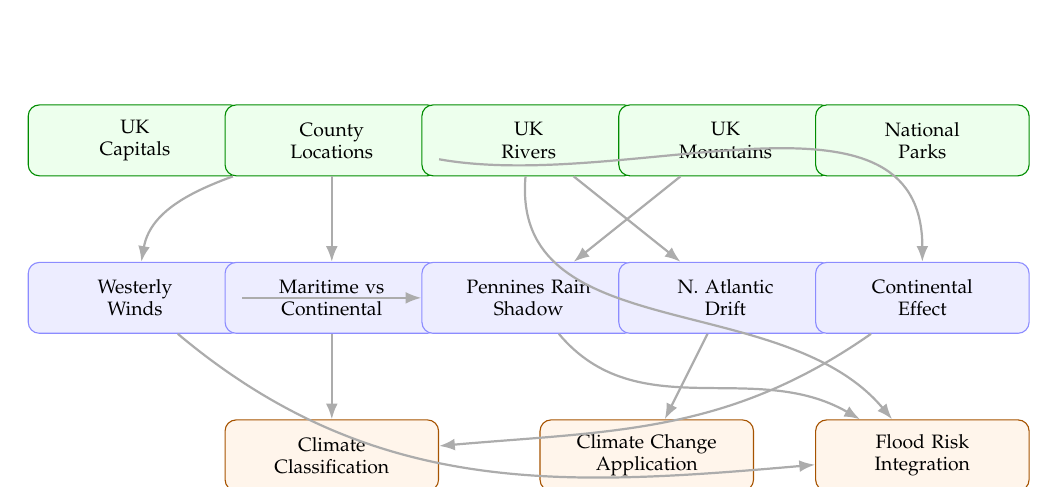
\begin{tikzpicture}[
  kc/.style={rectangle, rounded corners=4pt, draw=black!70,
    text width=2.5cm, align=center, font=\scriptsize,
    minimum height=0.9cm, inner sep=3pt},
  l1/.style={kc, fill=green!7, draw=green!55!black},
  l2/.style={kc, fill=blue!7, draw=blue!45},
  l3/.style={kc, fill=orange!8, draw=orange!65!black},
  arr/.style={-{Latex[length=2mm]}, gray!65, thick}
]

%% Level 1: Remembering (y = 4.5)
\node[l1] (caps)    at ( 0.0, 4.5) {UK\\Capitals};
\node[l1] (county)  at ( 2.5, 4.5) {County\\Locations};
\node[l1] (rivers)  at ( 5.0, 4.5) {UK\\Rivers};
\node[l1] (mnts)    at ( 7.5, 4.5) {UK\\Mountains};
\node[l1] (parks)   at (10.0, 4.5) {National\\Parks};

%% Level 2: Understanding (y = 2.5)
\node[l2] (westerly)    at ( 0.0, 2.5) {Westerly\\Winds};
\node[l2] (maritime)    at ( 2.5, 2.5) {Maritime vs\\Continental};
\node[l2] (pennines)    at ( 5.0, 2.5) {Pennines Rain\\Shadow};
\node[l2] (natldrift)   at ( 7.5, 2.5) {N.\ Atlantic\\Drift};
\node[l2] (continental) at (10.0, 2.5) {Continental\\Effect};

%% Level 3: Applying (y = 0.5)
\node[l3] (climclass)  at ( 2.5, 0.5) {Climate\\Classification};
\node[l3] (climchange) at ( 6.5, 0.5) {Climate Change\\Application};
\node[l3] (flood)      at (10.0, 0.5) {Flood Risk\\Integration};

%% L1 → L2
\draw[arr] (county) to[out=200,in=80]  (westerly);
\draw[arr] (county) --                 (maritime);
\draw[arr] (county) to[out=350,in=90]  (continental);
\draw[arr] (mnts)   --                 (pennines);
\draw[arr] (rivers) --                 (natldrift);

%% L2 → L2
\draw[arr] (westerly) -- (pennines);

%% L2 → L3
\draw[arr] (maritime)    -- (climclass);
\draw[arr] (continental) to[out=215,in=5]   (climclass);
\draw[arr] (natldrift)   -- (climchange);
\draw[arr] (pennines)    to[out=310,in=150]  (flood);

%% L1 → L3
\draw[arr] (rivers) to[out=265,in=130] (flood);

%% L2 → L3 (westerly winds → flood risk)
\draw[arr] (westerly) to[out=320,in=185] (flood);

\end{tikzpicture}
\caption{KC prerequisite DAG: 13 nodes across three Bloom levels
  (green~=~L1 Remembering, blue~=~L2 Understanding, orange~=~L3 Applying).
  Arrows indicate structural dependency; mastery gate
  $p(\text{Learned}) \geq 0.80$ on the prerequisite KC before
  dependent-KC items unlock. 12 edges total.}
\label{fig:kc_dag}
\end{figure}

% ─────────────────────────────────────────────────────────────────────────────
\section{Adaptive Algorithm Design}
\label{sec:meth_algorithms}
% ─────────────────────────────────────────────────────────────────────────────

\subsection{IRT 3PL Model}
\label{subsec:meth_irt}

The probability of a correct response from a learner with latent ability
$\theta$ on item $i$ is modelled by the 3PL function \parencite{birnbaum1968}:

\begin{equation}
  P(X=1 \mid \theta) = c_i + \frac{1-c_i}{1 + e^{-a_i(\theta - b_i)}}
  \label{eq:irt_3pl_meth}
\end{equation}

where $a_i \in [0.5, 3.0]$ is discrimination, $b_i \in [-3, 3]$ is difficulty,
and $c_i = 0.25$ is the pseudo-guessing parameter (fixed for four-option MCQs).
Parameters are calibrated offline using the \texttt{mirt} package in R
\parencite{chalmers2012} and serialised to JSON for Node.js consumption.

\subsection{EAP Ability Estimation}
\label{subsec:meth_eap}

Learner ability is updated after each response via Expected A Posteriori (EAP)
estimation \parencite{bock1982}:

\begin{equation}
  \hat{\theta}_{\text{EAP}} = \frac{\displaystyle\sum_{k=1}^{K}
    \theta_k \cdot L(\theta_k) \cdot \pi(\theta_k)}
    {\displaystyle\sum_{k=1}^{K} L(\theta_k) \cdot \pi(\theta_k)}
  \label{eq:eap_meth}
\end{equation}

where $K = 81$ grid points span $[-4, 4]$ with step $0.1$. The prior
$\pi(\theta_k) = \mathcal{N}(\mu_0, \sigma_0)$ is initialised at
$\mu_0 = -0.780$ (20th percentile) and $\sigma_0 = 0.543$. Following
pre-test seeding, the prior is tightened to $\sigma_0 = 0.35$.

\subsection{Bayesian Knowledge Tracing}
\label{subsec:meth_bkt}

Per-KC knowledge state is maintained as a BKT posterior \parencite{corbett1995},
updated after each response:

\begin{equation}
  p(L_n \mid \text{obs}_n) = \frac{P(\text{obs}_n \mid L_n) \cdot p(L_n)}
    {P(\text{obs}_n \mid L_n) \cdot p(L_n) + P(\text{obs}_n \mid \neg L_n)
    \cdot (1 - p(L_n))}
  \label{eq:bkt_update_meth}
\end{equation}

with learning transition $p(L_{n+1}) = p(L_n \mid \text{obs}_n) +
(1 - p(L_n \mid \text{obs}_n)) \cdot p(T)$.

\subsubsection*{Credit Factor Modification}

This project modifies the learning transition by a credit factor $\text{cf}$
reflecting the scaffolding level at which the correct response was obtained:

\begin{equation}
  p(L_{n+1})^* = p(L_n \mid \text{obs}_n) + \bigl(1 - p(L_n \mid
    \text{obs}_n)\bigr) \cdot p(T) \cdot \text{cf}
  \label{eq:bkt_credit_meth}
\end{equation}

\begin{table}[H]
\centering
\caption{Credit factor values by maximum hint level accessed per question.}
\label{tab:credit_factors}
\renewcommand{\arraystretch}{1.25}
\begin{tabular}{clc}
\toprule
\textbf{Max hint level} & \textbf{Scaffolding type} & \textbf{cf} \\
\midrule
0 & No hint accessed (unaided)         & 1.00 \\
1 & Conceptual reframe                 & 0.90 \\
2 & Procedural strategy hint           & 0.70 \\
3 & Worked example (full solution)     & 0.50 \\
\bottomrule
\end{tabular}
\end{table}

\subsection{Question Selection Algorithm}
\label{subsec:meth_selection}

At each step the adaptive engine selects from the eligible pool via a
multi-gate pipeline (Figure~\ref{fig:selection_flowchart}):
(1)~mastery gate: exclude KCs with unmastered prerequisites;
(2)~Bloom gate: exclude items above the learner's escalation threshold
(L2 unlocks at $p(\text{Learned}) \geq 0.40$ or prerequisite KC $\geq 0.50$;
L3 at $\geq 0.60$);
(3)~deduplication: exclude variants seen by this learner in any prior session;
(4)~decay boost: multiply Fisher information by $1.5$ for decayed KCs;
(5)~ZPD targeting: select $i^* = \arg\max_{i \in \mathcal{E}} I_i(\hat{\theta})$:

\begin{equation}
  i^* = \arg\max_{i \in \mathcal{E}}
    \frac{a_i^2 \cdot P_i(\hat{\theta})(1 - P_i(\hat{\theta}))}
    {\left(\dfrac{P_i(\hat{\theta}) - c_i}{1 - c_i}\right)^2}
  \label{eq:selection}
\end{equation}

If the eligible pool is exhausted, the engine falls back to the full
unrestricted pool and emits a \texttt{variant\_pool\_exhausted} event.

\begin{figure}[H]
\centering
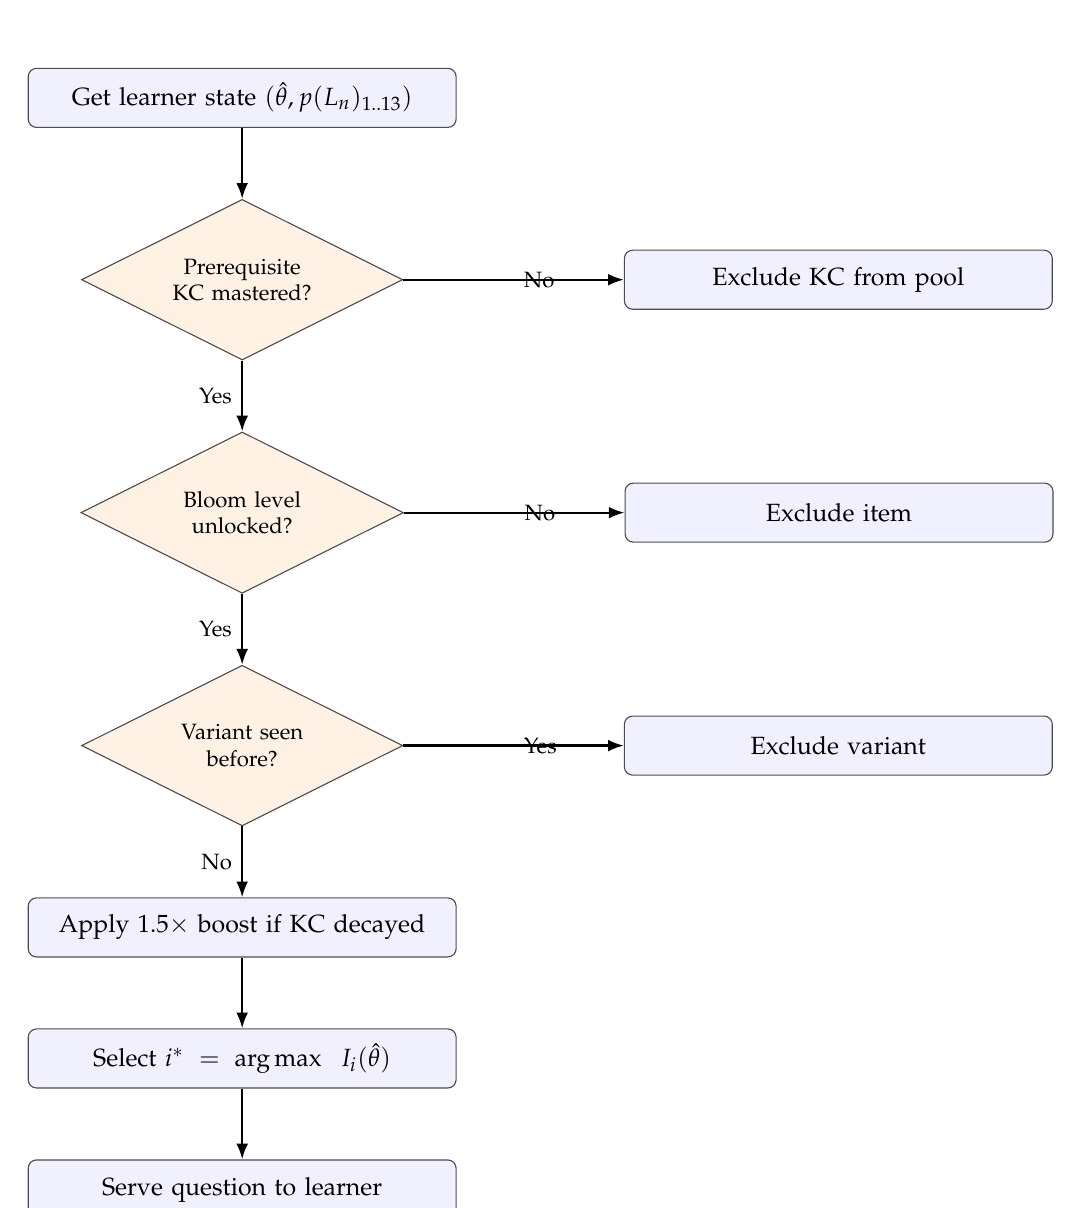
\begin{tikzpicture}[
  node distance=0.9cm,
  box/.style={rectangle, draw=black!70, rounded corners=3pt, text width=5.2cm,
    align=center, fill=blue!6, font=\small, minimum height=0.75cm},
  dec/.style={diamond, draw=black!70, fill=orange!10, text width=2.8cm,
    align=center, font=\footnotesize, inner sep=1pt, aspect=2},
  arr/.style={-{Latex[length=2mm]}, thick},
  yes/.style={font=\footnotesize, left},
  no/.style={font=\footnotesize, right}
]
\node[box] (start) {Get learner state $(\hat{\theta}, p(L_n)_{1..13})$};
\node[dec, below=of start] (mastery) {Prerequisite\\KC mastered?};
\node[box, right=2.8cm of mastery] (skip) {Exclude KC from pool};
\node[dec, below=of mastery] (bloom) {Bloom level\\unlocked?};
\node[box, right=2.8cm of bloom] (skipb) {Exclude item};
\node[dec, below=of bloom] (dedup) {Variant seen\\before?};
\node[box, right=2.8cm of dedup] (skipd) {Exclude variant};
\node[box, below=of dedup] (decay) {Apply $1.5\times$ boost if KC decayed};
\node[box, below=of decay] (fisher) {Select $i^* = \arg\max\; I_i(\hat{\theta})$};
\node[box, below=of fisher] (serve) {Serve question to learner};

\draw[arr] (start) -- (mastery);
\draw[arr] (mastery) -- node[yes]{Yes} (bloom);
\draw[arr] (mastery) -- node[no]{No} (skip);
\draw[arr] (bloom) -- node[yes]{Yes} (dedup);
\draw[arr] (bloom) -- node[no]{No} (skipb);
\draw[arr] (dedup) -- node[yes]{No} (decay);
\draw[arr] (dedup) -- node[no]{Yes} (skipd);
\draw[arr] (decay) -- (fisher);
\draw[arr] (fisher) -- (serve);
\end{tikzpicture}
\caption{Adaptive question selection flowchart. Steps execute in sequence per
question request.}
\label{fig:selection_flowchart}
\end{figure}

% ─────────────────────────────────────────────────────────────────────────────
\section{IRT Calibration Pipeline}
\label{subsec:meth_calibration}
% ─────────────────────────────────────────────────────────────────────────────

IRT item parameters are estimated via a two-stage offline pipeline.
(1)~The response matrix from a pilot study is exported from Supabase to CSV.
(2)~The \texttt{mirt} package \parencite{chalmers2012} fits the 3PL model
with $c_i$ constrained to $0.25$; convergence is verified using RMSEA
(acceptable: $< 0.08$). If 3PL estimation is unstable (RMSEA $> 0.10$ or
non-convergence within 500 EM cycles), the model falls back to Rasch (1PL).
(3)~Estimated $a_i$ and $b_i$ parameters are serialised to
\texttt{question\_bank.json} and committed to the repository for Node.js
runtime consumption.

% ─────────────────────────────────────────────────────────────────────────────
\section{Pre-Test Seeding}
\label{sec:meth_pretest}
% ─────────────────────────────────────────────────────────────────────────────

Before the adaptive session, a 13-item diagnostic pre-test (one item per KC
at Bloom Level~1) provides initial ability evidence, addressing the cold-start
problem \parencite{matos2025}. The raw score is converted to a Laplace-smoothed
logit seed:

\begin{equation}
  \theta_{\text{seed}} = \frac{\ln\!\left(\dfrac{n_{\text{correct}} + 0.5}
    {n_{\text{incorrect}} + 0.5}\right)}{1.7}
  \label{eq:theta_seed_meth}
\end{equation}

bounded to $[-2.5, 2.5]$, with the EAP prior standard deviation reduced to
$0.35$ to reflect additional information.

% ─────────────────────────────────────────────────────────────────────────────
\section{Scaffolding and Variant Design}
\label{sec:meth_scaffolding}
% ─────────────────────────────────────────────────────────────────────────────

Each question provides three graduated hint levels following
\textcite{koedinger2007}: Level~1 (conceptual reframe, no solution disclosure);
Level~2 (procedural strategy, method without answer); Level~3 (worked analogy,
cognitive pathway explicit). Each access reduces the credit factor applied to
a subsequent correct response (Table~\ref{tab:credit_factors}).

Each KC-Bloom combination is authored as a \texttt{Question\-Template} with
multiple \texttt{Question\-Variant} records substituting surface-level details
while preserving the underlying cognitive demand. Every variant served is
recorded in \texttt{User\-Variant\-Seen}, preventing re-exposure across sessions.
If all variants of a template are exhausted, the engine falls back to the
full template-level pool.

% ─────────────────────────────────────────────────────────────────────────────
\section{Evaluation Protocol}
\label{sec:meth_evaluation}
% ─────────────────────────────────────────────────────────────────────────────

\subsection{Study Design and Instruments}
\label{subsec:meth_study}

The evaluation uses a within-subjects quasi-experimental design. VanLehn's
(2011) meta-analytic benchmark of $d = 0.76$ serves as the primary comparison
standard; a direct no-adaptation control arm could not be completed within the
single-session constraint. Instruments administered include: the System Usability
Scale (SUS; 10-item Likert, scored 0--100, benchmark $\geq 68$
\parencite{bangor2008}); session-level $\hat{\theta}$ sequences for within-session
learning gain analysis; post-session distractor frequency tables for misconception
analysis; and a 7-day isomorphic retention assessment.

\subsection{Limitations of the Evaluation}
\label{subsec:meth_limitations}

\begin{itemize}[leftmargin=2em]
  \item \textbf{Sample size.} $n = 4$ external participants, substantially below
        the target of $n = 15$. Results are descriptive and proof-of-concept only;
        inferential statistics require approximately $n = 13$ for 80\% power at
        $d = 0.76$, $\alpha = 0.05$.
  \item \textbf{No control condition completed.} VanLehn's benchmark serves as
        the comparative reference.
  \item \textbf{Convenience sample.} University students are not representative
        of the KS3/GCSE student population.
  \item \textbf{IRT parameters from pilot.} Parameter instability is mitigated
        by the constrained calibration strategy.
\end{itemize}

% ─────────────────────────────────────────────────────────────────────────────
\section{System Architecture Overview}
\label{sec:meth_architecture}
% ─────────────────────────────────────────────────────────────────────────────

\begin{figure}[H]
\centering
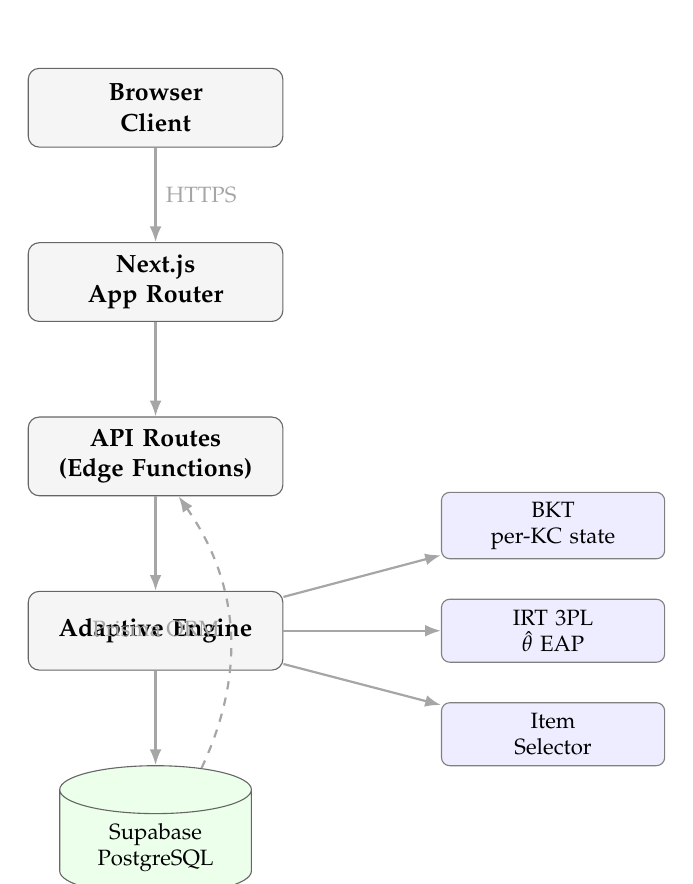
\begin{tikzpicture}[
  node distance=1.2cm and 1.8cm,
  layer/.style={rectangle, draw=black!60, rounded corners=4pt,
    fill=gray!8, text width=3.0cm, align=center,
    font=\small\bfseries, minimum height=1.0cm},
  mod/.style={rectangle, draw=black!50, rounded corners=3pt,
    fill=blue!7, text width=2.6cm, align=center,
    font=\footnotesize, minimum height=0.8cm},
  db/.style={cylinder, shape border rotate=90, draw=black!60,
    fill=green!8, text width=2.2cm, align=center,
    font=\footnotesize, minimum height=1.0cm, aspect=0.25},
  arr/.style={-{Latex[length=2mm]}, thick, gray!70}
]
\node[layer] (client) {Browser\\Client};
\node[layer, below=of client] (nextjs) {Next.js\\App Router};
\node[layer, below=of nextjs] (api) {API Routes\\(Edge Functions)};
\node[layer, below=of api] (engine) {Adaptive Engine};
\node[db, below=of engine] (db) {Supabase\\PostgreSQL};

\node[mod, right=2.0cm of engine] (irt) {IRT 3PL\\$\hat{\theta}$ EAP};
\node[mod, above=0.5cm of irt] (bkt) {BKT\\per-KC state};
\node[mod, below=0.5cm of irt] (sel) {Item\\Selector};

\draw[arr] (client) -- node[right, font=\footnotesize]{HTTPS} (nextjs);
\draw[arr] (nextjs) -- (api);
\draw[arr] (api) -- (engine);
\draw[arr] (engine) -- (db);
\draw[arr] (engine) -- (irt);
\draw[arr] (engine) -- (bkt);
\draw[arr] (engine) -- (sel);
\draw[arr, dashed] (db) to[bend right=30] node[left, font=\footnotesize]{Prisma ORM} (api);
\end{tikzpicture}
\caption{High-level system architecture. The adaptive engine is isolated as a
pure-function module with no direct database access; all I/O passes through
the API route layer.}
\label{fig:architecture}
\end{figure}

GeoMentor is deployed as a Next.js~14 (App Router) application on Vercel,
with Supabase (Frankfurt) providing PostgreSQL, Row-Level Security, and
authentication. Prisma ORM manages schema migrations and type-safe access.

% ─────────────────────────────────────────────────────────────────────────────
\section{Agile Development Methodology}
\label{sec:meth_agile}
% ─────────────────────────────────────────────────────────────────────────────

Development followed two-week sprints adapted from Scrum, managed through a
Notion project tracker. The iterative cycle was chosen because adaptive
algorithm design requires empirical validation: initial IRT parameter estimates
are hypotheses, not specifications, and multiple calibration cycles are needed
to stabilise. Table~\ref{tab:sprints} summarises the sprint history.

\begin{table}[H]
\centering
\caption{Sprint history: objectives, deliverables, and retrospective notes.}
\label{tab:sprints}
\renewcommand{\arraystretch}{1.25}
\begin{tabularx}{\textwidth}{clXX}
\toprule
\textbf{Sprint} & \textbf{Dates} & \textbf{Objective} & \textbf{Key deliverable / deviation} \\
\midrule
1 & Oct--Nov 2025 & Requirements, KC ontology, technology selection &
  13 KC prerequisite graph; technology ADRs (Next.js + Supabase) \\
2 & Nov--Dec 2025 & Core adaptive engine, database schema, pre-test seeding &
  \texttt{adaptive-engine.ts}; Prisma schema; EAP implementation \\
3 & Dec 2025--Jan 2026 & Question bank, IRT calibration pipeline, BKT &
  \texttt{seedKCs.ts} (13 KCs, 3 Bloom levels); R calibration script \\
4 & Jan--Feb 2026 & Scaffolding (hint system), variant deduplication &
  \texttt{hints/route.ts}; \texttt{UserVariantSeen} table; credit-factor BKT \\
5 & Feb 2026 & Scope reduction decision; evaluation redesign &
  Scope locked to single-KC validation; VanLehn benchmark adopted as comparator \\
6 & Feb--Mar 2026 & Session continuity, onboarding tour, pause/resume &
  \texttt{FirstVisitTour.tsx}; pause menu; session restore logic \\
7 & Mar 2026 & Security hardening (NIST 800-63B), rate limiting, RLS &
  Auth middleware; Supabase RLS policies; bcrypt migration \\
8 & Mar--Apr 2026 & Leaderboard, XP system, confidence calibration &
  \texttt{leaderboard/route.ts}; XP/level schema; decay notifications \\
9 & Apr 2026 & Evaluation data collection, SUS administration &
  SUS instrument deployed; participant sessions recorded \\
10 & Apr--May 2026 & Dissertation writing, final polishing &
  Dissertation LaTeX; this chapter \\
\bottomrule
\end{tabularx}
\end{table}

% ─────────────────────────────────────────────────────────────────────────────
\section{Project Timeline}
\label{sec:meth_gantt}
% ─────────────────────────────────────────────────────────────────────────────

Figure~\ref{fig:gantt} presents the planned and actual project timeline
reconstructed from the Git commit history.

\begin{figure}[H]
\centering
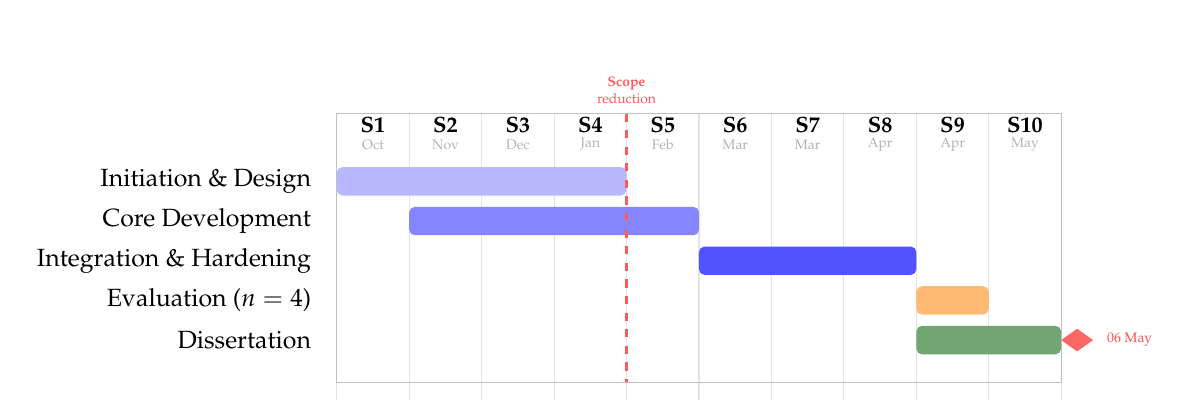
\begin{tikzpicture}[x=0.92cm, y=0.72cm]
  \foreach \x in {0,...,10} {
    \draw[gray!22, thin] (\x, 0.65) -- (\x, -4.60);
  }
  \foreach \i in {1,...,10} {
    \pgfmathsetmacro\xc{\i - 0.5}
    \node[font=\footnotesize\bfseries] at (\xc, 0.45) {S\i};
  }
  \foreach \xc/\mo in
      {0.5/Oct, 1.5/Nov, 2.5/Dec, 3.5/Jan, 4.5/Feb,
       5.5/Mar, 6.5/Mar, 7.5/Apr, 8.5/Apr, 9.5/May} {
    \node[font=\tiny, gray!60] at (\xc, 0.10) {\mo};
  }
  \fill[blue!28, rounded corners=2pt] (0,-0.30) rectangle (4,-0.80);
  \node[anchor=east, font=\small] at (-0.22,-0.55) {Initiation \& Design};
  \fill[blue!48, rounded corners=2pt] (1,-1.00) rectangle (5,-1.50);
  \node[anchor=east, font=\small] at (-0.22,-1.25) {Core Development};
  \fill[blue!68, rounded corners=2pt] (5,-1.70) rectangle (8,-2.20);
  \node[anchor=east, font=\small] at (-0.22,-1.95) {Integration \& Hardening};
  \fill[orange!55, rounded corners=2pt] (8,-2.40) rectangle (9,-2.90);
  \node[anchor=east, font=\small] at (-0.22,-2.65) {Evaluation ($n=4$)};
  \fill[green!35!black!55, rounded corners=2pt] (8,-3.10) rectangle (10,-3.60);
  \node[anchor=east, font=\small] at (-0.22,-3.35) {Dissertation};
  \draw[red!65, thick, dashed] (4, 0.65) -- (4,-4.10);
  \node[red!65, font=\tiny, align=center, above] at (4, 0.65)
      {\textbf{Scope}\\reduction};
  \fill[red!60]
      (10.00,-3.35) -- (10.22,-3.15) -- (10.44,-3.35) -- (10.22,-3.55) -- cycle;
  \node[anchor=west, font=\tiny, red!70] at (10.50,-3.35) {06~May};
  \draw[black!25] (0, 0.65) rectangle (10,-4.10);
\end{tikzpicture}
\caption{Project Gantt chart. Each column = one fortnightly sprint (Oct~2025--May~2026).
The red dashed line marks the Sprint~5 scope reduction.}
\label{fig:gantt}
\end{figure}

% ─────────────────────────────────────────────────────────────────────────────
\section{Risk Register}
\label{sec:meth_risks}
% ─────────────────────────────────────────────────────────────────────────────

\begin{table}[H]
\centering
\caption{Project risk register. L = Likelihood; I = Impact (H/M/L).}
\label{tab:risk_register}
\renewcommand{\arraystretch}{1.25}
\begin{tabularx}{\textwidth}{cp{4.0cm}ccp{2.0cm}X}
\toprule
\textbf{ID} & \textbf{Risk} & \textbf{L} & \textbf{I} & \textbf{Status} & \textbf{Mitigation} \\
\midrule
R1 & IRT 3PL fails to converge &
  H & M & Mitigated &
  Pre-specify Rasch fallback; fix $c=0.25$ \\
R2 & Participant attrition at follow-up &
  H & M & Accepted &
  Target $n=18$ recruitment; acknowledged in limitations \\
R3 & \texttt{variant\_pool\_\allowbreak exhausted} &
  M & L & Mitigated &
  Fallback to unrestricted pool; event emitted \\
R4 & Supabase RLS misconfiguration &
  L & H & Mitigated &
  RLS policies peer-reviewed; rate limiting on auth \\
R5 & BKT state corruption (concurrent sessions) &
  L & H & Mitigated &
  Postgres row-level locking; atomic session writes \\
R6 & Scope overrun (multi-domain) &
  H & H & Resolved &
  Sprint~5 scope reduction to single-domain Geography \\
\bottomrule
\end{tabularx}
\end{table}

% ─────────────────────────────────────────────────────────────────────────────
\section{What Was and Was Not Delivered}
\label{sec:meth_delivery}
% ─────────────────────────────────────────────────────────────────────────────

\subsection{Delivered}

\begin{itemize}[leftmargin=2em]
  \item Hybrid IRT 3PL + BKT adaptive engine with EAP estimation,
        Bloom-gated selection, and credit-factor BKT modification
  \item 13-KC question bank with isomorphic variants and cross-session deduplication
  \item Three-level graduated hint system with evidential credit weighting
  \item Pre-test seeding with Laplace-smoothed logit initialisation
  \item BKT decay detection and successive relearning boost ($1.5\times$)
  \item Five-tab session summary dashboard (Trajectory, Skills, Misconceptions, Achievements, Share)
  \item Leaderboard with XP ranking, consent opt-in, and rank-change animation
  \item First-visit onboarding tour
  \item Security implementation: bcrypt, JWT, rate limiting, Supabase RLS, NIST SP 800-63B compliance
  \item Production deployment on Vercel with Supabase Frankfurt backend
\end{itemize}

\subsection{Not Delivered}

\begin{itemize}[leftmargin=2em]
  \item \textbf{Multi-domain support.} Superseded by the Sprint~5 scope
        reduction; the architecture supports extension without algorithmic change.
  \item \textbf{K-means cold-start clustering.} Evaluated and superseded by
        pre-test seeding, which provides per-KC ability evidence rather than
        a demographic cluster assignment.
  \item \textbf{Full A/B randomised controlled trial.} VanLehn's meta-analytic
        benchmark used as comparator; static arm implemented but not wired.
  \item \textbf{7-day retention data at scale.} Follow-up data collection could
        not be completed within the project timeline.
\end{itemize}

% ─────────────────────────────────────────────────────────────────────────────
\section{Interface Design: Lo-fi Prototypes}
\label{sec:meth_lofi}
% ─────────────────────────────────────────────────────────────────────────────

Interface design preceded implementation in each sprint cycle.
Figure~\ref{fig:lofi_question} shows the lo-fi wireframe for the adaptive
question screen, and Figure~\ref{fig:lofi_summary} shows the session summary
dashboard layout. Both informed the production React component specifications
authored by the candidate.

\begin{figure}[H]
\centering
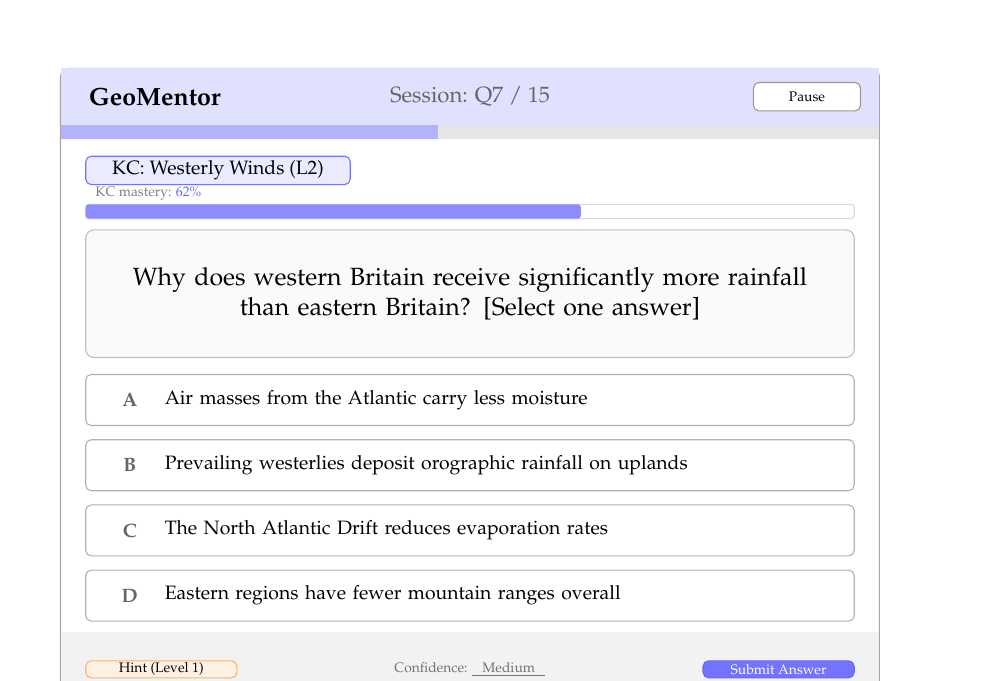
\begin{tikzpicture}[x=0.80cm, y=0.72cm]
  % Outer browser chrome
  \draw[black!35, rounded corners=3pt] (0,0) rectangle (13,-11);

  % Top navigation bar
  \fill[blue!12] (0,0) rectangle (13,-1.0);
  \node[anchor=west, font=\small\bfseries] at (0.3,-0.50) {GeoMentor};
  \node[font=\footnotesize, black!60] at (6.5,-0.50) {Session: Q7 / 15};
  \draw[black!40, rounded corners=2pt, fill=white] (11.0,-0.75) rectangle (12.7,-0.25);
  \node[font=\tiny] at (11.85,-0.50) {Pause};

  % Progress bar strip
  \fill[blue!30] (0,-1.0) rectangle (6.0,-1.25);
  \fill[gray!20] (6.0,-1.0) rectangle (13,-1.25);

  % KC badge + Bloom level
  \draw[blue!55, rounded corners=2pt, fill=blue!8]
    (0.4,-1.55) rectangle (4.6,-2.05);
  \node[font=\scriptsize] at (2.5,-1.80) {KC: Westerly Winds (L2)};

  % Mastery bar label
  \node[font=\tiny, black!50, anchor=west] at (0.4,-2.20)
    {KC mastery: {\color{blue!60}62\%}};
  \draw[gray!30, rounded corners=1pt] (0.4,-2.40) rectangle (12.6,-2.65);
  \fill[blue!45, rounded corners=1pt] (0.4,-2.40) rectangle (8.26,-2.65);

  % Question text box
  \draw[black!25, rounded corners=3pt, fill=gray!4]
    (0.4,-2.85) rectangle (12.6,-5.10);
  \node[font=\small, align=center, text width=11cm] at (6.5,-3.97)
    {Why does western Britain receive significantly more rainfall\\
     than eastern Britain? [Select one answer]};

  % Answer options
  \foreach \i/\lbl/\txt in {
    0/A/Air masses from the Atlantic carry less moisture,
    1/B/Prevailing westerlies deposit orographic rainfall on uplands,
    2/C/The North Atlantic Drift reduces evaporation rates,
    3/D/Eastern regions have fewer mountain ranges overall
  }{
    \pgfmathsetmacro\yy{-5.40 - \i*1.15}
    \draw[black!30, rounded corners=2pt, fill=white]
      (0.4,\yy) rectangle (12.6,\yy-0.90);
    \node[font=\scriptsize\bfseries, black!60] at (1.1,\yy-0.45) {\lbl};
    \node[font=\scriptsize, anchor=west, text width=10cm] at (1.5,\yy-0.45) {\txt};
  }

  % Bottom bar: Hint | Confidence | Submit
  \fill[gray!10] (0,-9.95) rectangle (13,-11);
  \draw[orange!60, rounded corners=2pt, fill=orange!10]
    (0.4,-10.45) rectangle (2.8,-10.75);
  \node[font=\tiny] at (1.6,-10.60) {Hint (Level 1)};
  \node[font=\tiny, black!55] at (6.5,-10.60)
    {Confidence: \underline{~~~Medium~~~}};
  \draw[blue!60, rounded corners=2pt, fill=blue!55]
    (10.2,-10.45) rectangle (12.6,-10.75);
  \node[font=\tiny, white] at (11.4,-10.60) {Submit Answer};
\end{tikzpicture}
\caption{Lo-fi wireframe: adaptive question screen. Key elements are the KC
  badge (identifies active Knowledge Component and Bloom level), the BKT
  mastery bar (reflects live $p(\text{Learned})$), four MCQ options, the
  graduated hint trigger (orange), confidence rating, and submit button.
  This wireframe preceded the Sprint~4 React implementation.}
\label{fig:lofi_question}
\end{figure}

\begin{figure}[H]
\centering
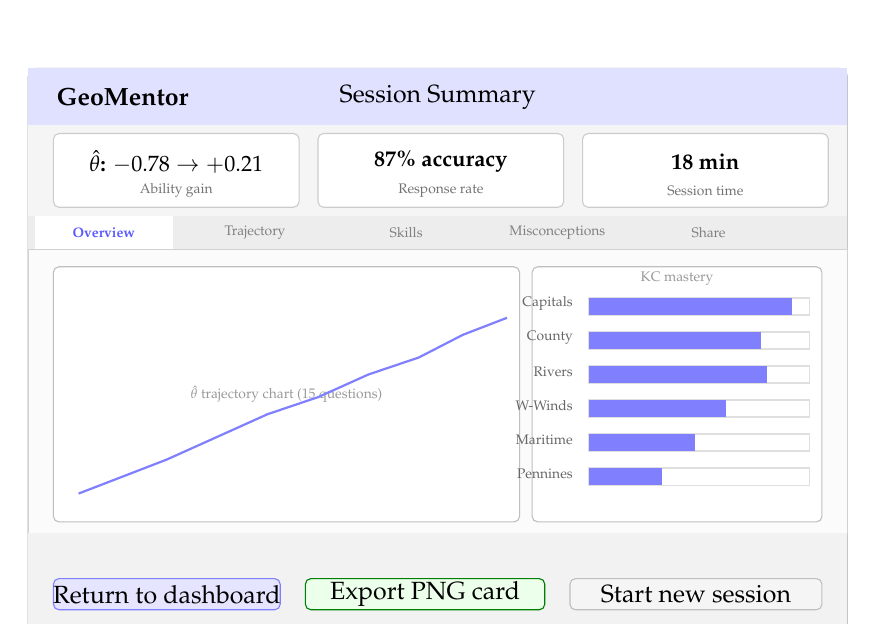
\begin{tikzpicture}[x=0.80cm, y=0.72cm]
  % Outer browser chrome
  \draw[black!35, rounded corners=3pt] (0,0) rectangle (13,-10);

  % Header bar
  \fill[blue!12] (0,0) rectangle (13,-1.0);
  \node[anchor=west, font=\small\bfseries] at (0.3,-0.50) {GeoMentor};
  \node[font=\small] at (6.5,-0.50) {Session Summary};

  % Stats strip: three stat boxes
  \fill[gray!8] (0,-1.0) rectangle (13,-2.6);
  \foreach \i/\statval/\statlbl in {
    0/{$\hat{\theta}$: $-0.78 \to +0.21$}/Ability gain,
    1/{87\% accuracy}/Response rate,
    2/{18 min}/Session time
  }{
    \pgfmathsetmacro\xleft{0.4 + \i*4.2}
    \pgfmathsetmacro\xright{\xleft + 3.9}
    \draw[black!20, rounded corners=2pt, fill=white]
      (\xleft,-1.15) rectangle (\xright,-2.45);
    \node[font=\footnotesize\bfseries] at (\xleft+1.95,-1.65) {\statval};
    \node[font=\tiny, black!55] at (\xleft+1.95,-2.15) {\statlbl};
  }

  % Tab bar
  \fill[gray!14] (0,-2.6) rectangle (13,-3.2);
  \foreach \i/\tabnm in {
    0/Overview, 1/Trajectory, 2/Skills, 3/Misconceptions, 4/Share
  }{
    \pgfmathsetmacro\tcx{1.2 + \i*2.4}
    \ifnum\i=0
      \fill[white] (\tcx-1.1,-2.6) rectangle (\tcx+1.1,-3.2);
      \node[font=\tiny\bfseries, blue!65] at (\tcx,-2.90) {\tabnm};
    \else
      \node[font=\tiny, black!50] at (\tcx,-2.90) {\tabnm};
    \fi
  }

  % Main content pane (Overview tab active)
  \draw[black!18, fill=gray!3] (0,-3.2) rectangle (13,-8.2);

  % Left: $\hat\theta$ trajectory chart placeholder
  \draw[black!25, fill=white, rounded corners=2pt]
    (0.4,-3.5) rectangle (7.8,-8.0);
  \node[font=\tiny, black!40] at (4.1,-5.75)
    {$\hat{\theta}$ trajectory chart (15 questions)};
  % Simulated line
  \draw[blue!50, thick]
    (0.8,-7.5) -- (1.5,-7.2) -- (2.2,-6.9) -- (3.0,-6.5)
    -- (3.8,-6.1) -- (4.6,-5.8) -- (5.4,-5.4) -- (6.2,-5.1)
    -- (6.9,-4.7) -- (7.6,-4.4);

  % Right: per-KC mastery bars
  \draw[black!25, fill=white, rounded corners=2pt]
    (8.0,-3.5) rectangle (12.6,-8.0);
  \node[font=\tiny, black!40, align=center] at (10.3,-3.70)
    {KC mastery};
  \foreach \j/\kcshort/\pct in {
    0/Capitals/0.92,
    1/County/0.78,
    2/Rivers/0.81,
    3/W-Winds/0.62,
    4/Maritime/0.48,
    5/Pennines/0.33
  }{
    \pgfmathsetmacro\ybase{-4.00 - \j*0.60}
    \node[anchor=east, font=\tiny, black!60] at (8.8,\ybase-0.15) {\kcshort};
    \draw[gray!25] (8.9,\ybase-0.05) rectangle (12.4,\ybase-0.35);
    \pgfmathsetmacro\barend{8.9 + \pct*3.5}
    \fill[blue!50] (8.9,\ybase-0.05) rectangle (\barend,\ybase-0.35);
  }

  % Bottom action bar
  \fill[gray!10] (0,-8.2) rectangle (13,-10);
  \draw[blue!50, rounded corners=2pt, fill=blue!10]
    (0.4,-9.0) rectangle (4.0,-9.55);
  \node[font=\small] at (2.2,-9.275) {Return to dashboard};
  \draw[green!50!black, rounded corners=2pt, fill=green!8]
    (4.4,-9.0) rectangle (8.2,-9.55);
  \node[font=\small] at (6.3,-9.275) {Export PNG card};
  \draw[gray!50, rounded corners=2pt, fill=gray!8]
    (8.6,-9.0) rectangle (12.6,-9.55);
  \node[font=\small] at (10.6,-9.275) {Start new session};
\end{tikzpicture}
\caption{Lo-fi wireframe: session summary dashboard (Overview tab active).
  The three-stat strip reports the within-session $\Delta\hat{\theta}$,
  overall accuracy, and session duration. Left pane: $\hat{\theta}$ trajectory
  chart across 15 questions. Right pane: per-KC BKT mastery bars.
  Tab navigation exposes Trajectory (interactive chart), Skills (KC breakdown),
  Misconceptions (distractor analysis), and Share (PNG card export).}
\label{fig:lofi_summary}
\end{figure}

% ─────────────────────────────────────────────────────────────────────────────
\section{Quality Assurance}
\label{sec:meth_qa}
% ─────────────────────────────────────────────────────────────────────────────

Quality assurance mechanisms employed include: TypeScript strict mode
eliminating runtime errors at the type-checking stage; Prisma migration files
providing a versioned schema audit trail; Vercel preview deployments enabling
integration testing per feature branch before merge; and Supabase RLS
verification by cross-user access testing from a test account.

\chapter{Implementation}
\label{ch:implementation}

% ─────────────────────────────────────────────────────────────────────────────
\section{System Architecture}
\label{sec:impl_architecture}
% ─────────────────────────────────────────────────────────────────────────────

GeoMentor is implemented as a monolithic Next.js~14 application deployed to
Vercel's edge network, with Supabase PostgreSQL hosted in the Frankfurt
(eu-central-1) region. The monolithic architecture was a deliberate decision:
the research contribution lies in the adaptive algorithm, not distributed
systems complexity, and a monolith reduces operational overhead and eliminates
inter-service latency. The key architectural constraint is the \textbf{isolation
of the adaptive engine}: the algorithm modules (\texttt{irt.ts} and
\texttt{bkt.ts}) are implemented as pure functions with no direct database
access. All database I/O passes through Next.js API route handlers, which
orchestrate the learner state lifecycle: loading state, invoking engine
functions, persisting updated state, and returning the question. This isolation
makes the engine independently testable and domain-agnostic.

Figure~\ref{fig:component_diagram} shows the four-layer component architecture;
Figure~\ref{fig:sequence_diagram} shows the question lifecycle across both
routes; Figure~\ref{fig:er_diagram} shows the core database schema.

\begin{table}[H]
\centering
\caption{Technology stack with architectural justification.}
\label{tab:tech_stack}
\renewcommand{\arraystretch}{1.25}
\begin{tabularx}{\textwidth}{llX}
\toprule
\textbf{Layer} & \textbf{Technology} & \textbf{Justification} \\
\midrule
Frontend & Next.js 14 (App Router) &
  React Server Components reduce client bundle size; streaming enables
  progressive session summary loading \\
Styling & Tailwind CSS &
  Utility-first CSS; consistent design tokens across all components \\
ORM & Prisma 5 &
  Type-safe database access; migration history provides schema audit trail \\
Database & Supabase PostgreSQL &
  Row-Level Security enforces data isolation at the database layer \\
Auth & Supabase Auth + JWT &
  PKCE flow; bcrypt password hashing; NIST SP 800-63B compliant \\
Deployment & Vercel &
  Preview deployments per branch; automatic HTTPS; edge caching \\
IRT calibration & R + \texttt{mirt} &
  Industry-standard psychometric tooling; offline and audit-logged \\
\bottomrule
\end{tabularx}
\end{table}

The system targets the following non-functional properties: \textbf{scalability}
via Vercel's serverless function infrastructure (each API route invocation is
an independent function execution); \textbf{reliability} via Supabase Frankfurt's
managed PostgreSQL cluster with daily automated backups; \textbf{efficiency}
with EAP grid integration and BKT update executing in-process within the API
route, targeting end-to-end question selection latency under 500\,ms; and
\textbf{maintainability} via TypeScript strict mode, Prisma migration files,
and the adaptive engine's pure-function architecture.

\begin{figure}[H]
\centering
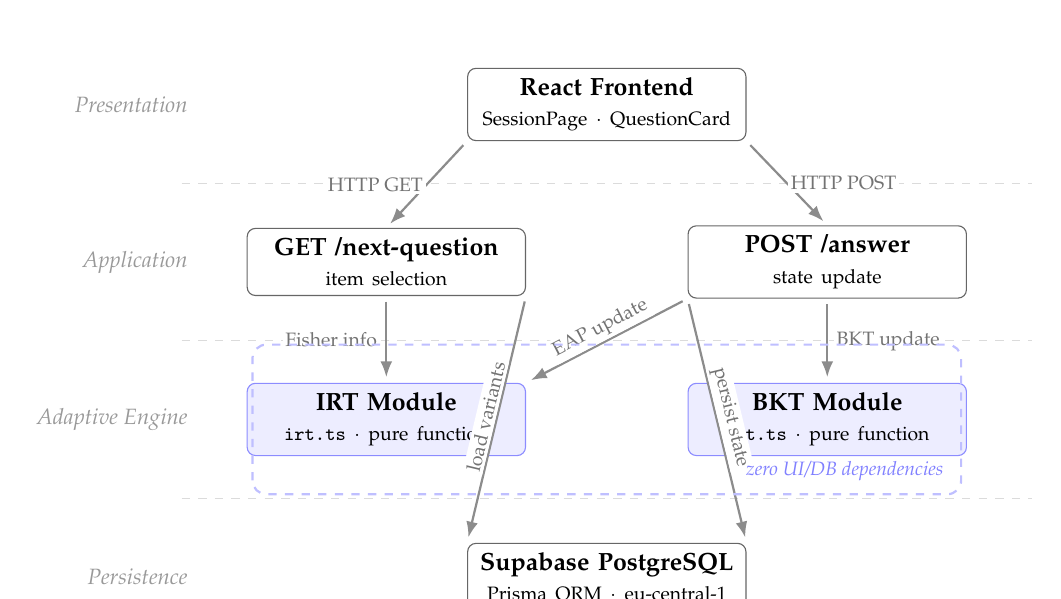
\begin{tikzpicture}[
  box/.style={rectangle, rounded corners=3pt, draw=black!60, fill=white,
              text width=3.3cm, minimum height=0.85cm, align=center, font=\small},
  engine/.style={box, fill=blue!7, draw=blue!45},
  arr/.style={-{Latex[length=2mm]}, thick, black!45, shorten >=2pt, shorten <=2pt},
  lbl/.style={font=\scriptsize, black!55, fill=white, inner sep=1pt}
]
\draw[black!14, dashed] (-5.4, 5.0) -- (5.4, 5.0);
\draw[black!14, dashed] (-5.4, 3.0) -- (5.4, 3.0);
\draw[black!14, dashed] (-5.4, 1.0) -- (5.4, 1.0);

\node[anchor=east, font=\footnotesize\itshape, text=black!40] at (-5.2, 6.0) {Presentation};
\node[anchor=east, font=\footnotesize\itshape, text=black!40] at (-5.2, 4.0) {Application};
\node[anchor=east, font=\footnotesize\itshape, text=black!40] at (-5.2, 2.0) {Adaptive Engine};
\node[anchor=east, font=\footnotesize\itshape, text=black!40] at (-5.2, 0.0) {Persistence};

\node[box] (fe) at (0, 6.0)
  {\textbf{React Frontend}\\{\scriptsize SessionPage $\cdot$ QuestionCard}};
\node[box] (nq) at (-2.8, 4.0)
  {\textbf{GET /next-question}\\{\scriptsize item selection}};
\node[box] (an) at (2.8, 4.0)
  {\textbf{POST /answer}\\{\scriptsize state update}};
\node[engine] (irt) at (-2.8, 2.0)
  {\textbf{IRT Module}\\{\scriptsize \texttt{irt.ts} $\cdot$ pure function}};
\node[engine] (bkt) at (2.8, 2.0)
  {\textbf{BKT Module}\\{\scriptsize \texttt{bkt.ts} $\cdot$ pure function}};
\node[box] (db) at (0, 0.0)
  {\textbf{Supabase PostgreSQL}\\{\scriptsize Prisma ORM $\cdot$ eu-central-1}};

\draw[arr] (fe.south west) -- node[lbl, left]{HTTP GET} (nq.north);
\draw[arr] (fe.south east) -- node[lbl, right]{HTTP POST} (an.north);
\draw[arr] (nq) -- node[lbl, left=2pt]{Fisher info} (irt);
\draw[arr] (an.south west) -- node[lbl, above, sloped]{EAP update} (irt.north east);
\draw[arr] (an) -- node[lbl, right=2pt]{BKT update} (bkt);
\draw[arr] (nq.south east) -- node[lbl, above, sloped]{load variants} (db.north west);
\draw[arr] (an.south west) -- node[lbl, above, sloped]{persist state} (db.north east);
\draw[blue!25, thick, dashed, rounded corners=5pt]
  (-4.5, 1.05) rectangle (4.5, 2.95);
\node[font=\scriptsize\itshape, text=blue!50, anchor=south east] at (4.4, 1.1)
  {zero UI/DB dependencies};
\end{tikzpicture}
\caption{UML 2.5 component diagram. The Adaptive Engine subsystem (IRT and BKT
modules) is implemented as pure functions with no direct UI or database
dependencies.}
\label{fig:component_diagram}
\end{figure}

% ─────────────────────────────────────────────────────────────────────────────
\section{Database Schema}
\label{sec:impl_schema}
% ─────────────────────────────────────────────────────────────────────────────

The Prisma schema defines 20 models. The six central to the adaptive engine
are described here; the full schema is in the repository
(\texttt{prisma/schema.prisma}).

The \textbf{Session} model carries the principal adaptive state: \texttt{theta}
(current EAP estimate, initialised at $-0.780$), \texttt{thetaSd} (posterior
SD, initialised at $0.543$), and \texttt{kcStates} (JSON-serialised
\texttt{Record<kcId, KCState>} carrying BKT state for all 13 KCs). JSON
serialisation eliminates join overhead on the hot adaptive selection path.
The \textbf{Interaction} model records every question--answer event with full
psychometric resolution: \texttt{theta\_before}/\texttt{theta\_after},
\texttt{pLearned\_before}/\texttt{pLearned\_after}, \texttt{hintLevelMax}
(used by the credit factor computation), and \texttt{responseTimeMs}.
The question bank is a two-layer hierarchy: \texttt{QuestionTemplate}
(defines KC, Bloom level, IRT parameters $a$, $b$, $c$, and a stem with
\texttt{\{variable\}} placeholders) and \texttt{QuestionVariant} (surface-specific
substitutions). \texttt{UserVariantSeen} records every (user, variant) pair
presented, enforced as a unique constraint to prevent re-exposure. The
\texttt{AnalyticsEvent} model provides a structured event log including
\texttt{bloom\_escalation}, \texttt{variant\_pool\_exhausted},
\texttt{kc\_mastered}, and \texttt{decay\_detected} events.

\begin{figure}[H]
\centering
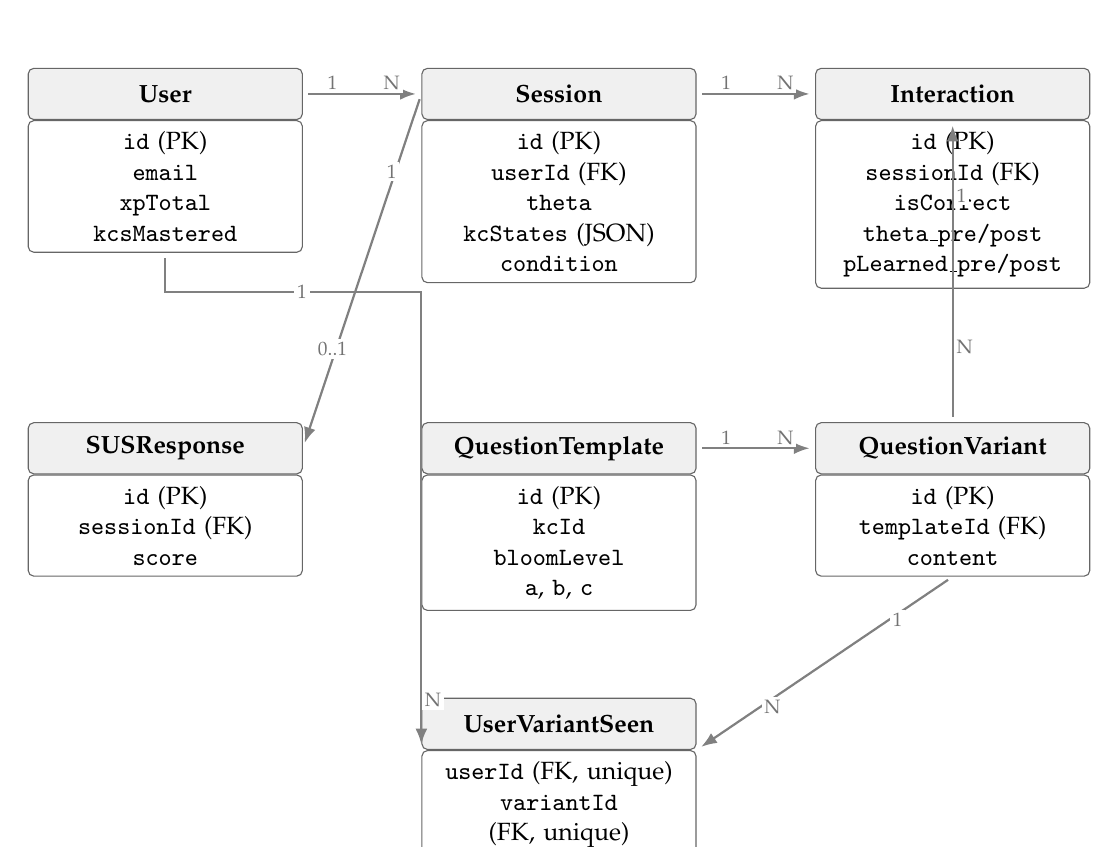
\begin{tikzpicture}[
  ent/.style={rectangle, draw=black!60, fill=white, rounded corners=2pt,
              text width=3.2cm, align=center, font=\small, inner sep=4pt},
  hdr/.style={ent, fill=gray!12, font=\small\bfseries, minimum height=0.65cm},
  arr/.style={-{Latex[length=2mm]}, thick, black!50, shorten >=2pt, shorten <=2pt},
  lbl/.style={font=\scriptsize, black!55, fill=white, inner sep=1pt}
]

\node[hdr] (uH) at (0, 8)      {User};
\node[ent, anchor=north] (u) at (uH.south) {
  \texttt{id} (PK)\\
  \texttt{email}\\
  \texttt{xpTotal}\\
  \texttt{kcsMastered}
};

\node[hdr] (sH) at (5, 8)      {Session};
\node[ent, anchor=north] (s) at (sH.south) {
  \texttt{id} (PK)\\
  \texttt{userId} (FK)\\
  \texttt{theta}\\
  \texttt{kcStates} (JSON)\\
  \texttt{condition}
};

\node[hdr] (iH) at (10, 8)     {Interaction};
\node[ent, anchor=north] (i) at (iH.south) {
  \texttt{id} (PK)\\
  \texttt{sessionId} (FK)\\
  \texttt{isCorrect}\\
  \texttt{theta\_pre/post}\\
  \texttt{pLearned\_pre/post}
};

\node[hdr] (tH) at (5, 3.5)    {QuestionTemplate};
\node[ent, anchor=north] (t) at (tH.south) {
  \texttt{id} (PK)\\
  \texttt{kcId}\\
  \texttt{bloomLevel}\\
  \texttt{a}, \texttt{b}, \texttt{c}
};

\node[hdr] (vH) at (10, 3.5)   {QuestionVariant};
\node[ent, anchor=north] (v) at (vH.south) {
  \texttt{id} (PK)\\
  \texttt{templateId} (FK)\\
  \texttt{content}
};

\node[hdr] (uvH) at (5, 0)     {UserVariantSeen};
\node[ent, anchor=north] (uv) at (uvH.south) {
  \texttt{userId} (FK, unique)\\
  \texttt{variantId} (FK, unique)
};

\node[hdr] (susH) at (0, 3.5)  {SUSResponse};
\node[ent, anchor=north] (sus) at (susH.south) {
  \texttt{id} (PK)\\
  \texttt{sessionId} (FK)\\
  \texttt{score}
};

\draw[arr] (uH.east) -- node[lbl, near start, above]{1}
                         node[lbl, near end,   above]{N} (sH.west);
\draw[arr] (sH.east) -- node[lbl, near start, above]{1}
                         node[lbl, near end,   above]{N} (iH.west);
\draw[arr] (tH.east) -- node[lbl, near start, above]{1}
                         node[lbl, near end,   above]{N} (vH.west);
\draw[arr] (vH.north) -- node[lbl, near start, right]{N}
                          node[lbl, near end,   right]{1} (iH.south);
\draw[arr] (u.south) -- ++(0,-0.5) -| (uv.north west)
  node[lbl, near start, right]{1};
\node[lbl] at (3.4, 0.3) {N};
\draw[arr] (v.south) -- node[lbl, near start, right]{1}
                         node[lbl, near end,   right]{N} (uv.north east);
\draw[arr] (sH.west) -- node[lbl, near start, above]{1}
                         node[lbl, near end,   above]{0..1} (susH.east);
\end{tikzpicture}
\caption[ER diagram: six core Prisma schema models.]{Entity-relationship diagram for the six core Prisma schema models.
\texttt{UserVariantSeen} enforces a unique (userId, variantId) constraint,
preventing variant re-exposure across sessions.}
\label{fig:er_diagram}
\end{figure}

% ─────────────────────────────────────────────────────────────────────────────
\section{Adaptive Engine Implementation}
\label{sec:impl_engine}
% ─────────────────────────────────────────────────────────────────────────────

The IRT module (\texttt{src/lib/algorithms/irt.ts}) implements the 3PL model
with the $D = 1.7$ logistic approximation \parencite{lord1980}. The EAP
estimator integrates over a grid of $K = 161$ points spanning $\theta \in
[-4, 4]$ with step $0.05$. The finer grid (compared to the $0.1$-step grid
specified at design time) was adopted after self-pilot testing revealed that
coarser grids produced visible staircase artefacts in the $\hat{\theta}$
trajectory for high-ability learners.

The BKT module (\texttt{src/lib/algorithms/bkt.ts}) implements the standard
Corbett--Anderson update plus the credit factor modification. The implementation
adopts a \textit{soft observation} interpolation: for credit-weighted correct
responses, the posterior is interpolated between the full Bayesian update and
the prior in proportion to $\text{cf}$, which is mathematically equivalent to
a Bayesian update with a degraded likelihood but numerically more stable.
Incorrect responses following hint access receive full-weight Bayesian updates:
providing a hint does not make an incorrect response less informative about
knowledge state.

The BKT mastery threshold is implemented at $p(\text{Learned}) \geq 0.95$,
higher than the $0.80$ threshold cited in the literature review. The binary
nature of BKT's latent state demands a stronger guarantee that the posterior
is not merely elevated by a lucky guess run. The $0.80$ threshold applies
separately to the IRT-based mastery check (\texttt{checkMastery()} in
\texttt{irt.ts}), which averages $P(\text{correct})$ across all KC items at
the current $\hat{\theta}$ using the continuous IRT scale.

% ─────────────────────────────────────────────────────────────────────────────
\section{API Route Design}
\label{sec:impl_api}
% ─────────────────────────────────────────────────────────────────────────────

The adaptive session is managed by four API routes. \textbf{GET
/api/sessions/[id]/next-question}: loads session state; builds the eligible
variant pool (joining \texttt{QuestionTemplate} and \texttt{QuestionVariant}
minus \texttt{UserVariantSeen}); applies mastery gate, Bloom gate, deduplication,
and decay boost; selects $i^* = \arg\max I_i(\hat{\theta})$; renders variant
by interpolating placeholders and shuffling answer options (Fisher-Yates);
returns serialised question object. \textbf{POST /api/sessions/[id]/answer}:
validates the submitted answer; computes credit factor from \texttt{hintLevelMax};
runs EAP update and BKT update; persists updated session state atomically;
writes \texttt{Interaction} record; checks mastery and Bloom escalation
thresholds; emits analytics events as appropriate.
\textbf{GET /api/sessions/[id]/summary}: generates the five-tab dashboard payload.
\textbf{GET /api/sessions/[id]/trajectory}: returns the longitudinal
$\hat{\theta}$ sequence for the ability progression chart. Figure~\ref{fig:sequence_diagram}
illustrates the complete question lifecycle.

\begin{figure}[H]
\centering
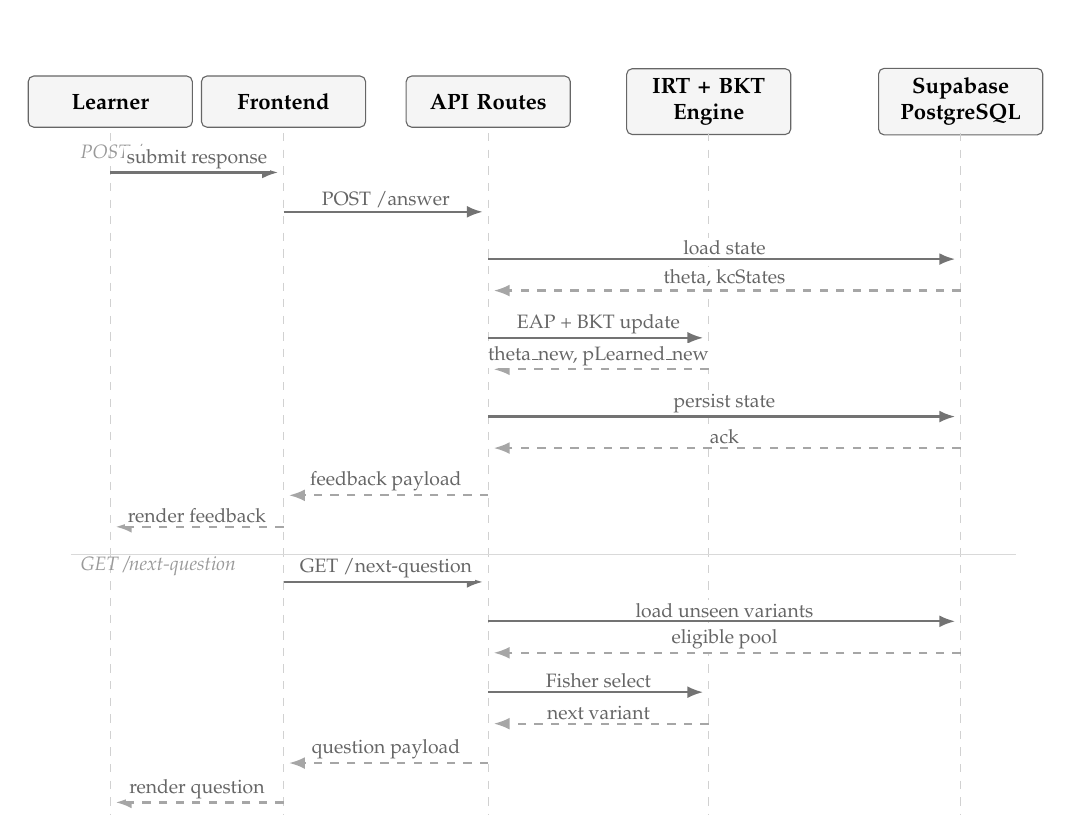
\begin{tikzpicture}[
  actor/.style={rectangle, rounded corners=2pt, draw=black!60, fill=gray!8,
                text width=1.85cm, minimum height=0.65cm, align=center,
                font=\footnotesize\bfseries},
  msg/.style={-{Latex[length=2mm]}, thick, black!55, shorten >=2pt},
  ret/.style={-{Latex[length=2mm]}, thick, black!35, dashed, shorten >=2pt},
  lbl/.style={font=\scriptsize, black!60, fill=white, inner sep=1pt}
]
\def\xL{0}
\def\xF{2.2}
\def\xA{4.8}
\def\xE{7.6}
\def\xD{10.8}

\node[actor] at (\xL, 9.5) {Learner};
\node[actor] at (\xF, 9.5) {Frontend};
\node[actor] at (\xA, 9.5) {API Routes};
\node[actor] at (\xE, 9.5) {IRT + BKT\\Engine};
\node[actor] at (\xD, 9.5) {Supabase\\PostgreSQL};

\draw[black!18, dashed] (\xL, 9.1) -- (\xL, 0.3);
\draw[black!18, dashed] (\xF, 9.1) -- (\xF, 0.3);
\draw[black!18, dashed] (\xA, 9.1) -- (\xA, 0.3);
\draw[black!18, dashed] (\xE, 9.1) -- (\xE, 0.3);
\draw[black!18, dashed] (\xD, 9.1) -- (\xD, 0.3);

\node[anchor=west, font=\scriptsize\itshape, text=black!40] at (-0.5, 8.85)
  {POST /answer};

\draw[msg] (\xL, 8.6) -- (\xF, 8.6)
  node[lbl, midway, above]{submit response};
\draw[msg] (\xF, 8.1) -- (\xA, 8.1)
  node[lbl, midway, above]{POST /answer};
\draw[msg] (\xA, 7.5) -- (\xD, 7.5)
  node[lbl, midway, above]{load state};
\draw[ret] (\xD, 7.1) -- (\xA, 7.1)
  node[lbl, midway, above]{theta, kcStates};
\draw[msg] (\xA, 6.5) -- (\xE, 6.5)
  node[lbl, midway, above]{EAP + BKT update};
\draw[ret] (\xE, 6.1) -- (\xA, 6.1)
  node[lbl, midway, above]{theta\_new, pLearned\_new};
\draw[msg] (\xA, 5.5) -- (\xD, 5.5)
  node[lbl, midway, above]{persist state};
\draw[ret] (\xD, 5.1) -- (\xA, 5.1)
  node[lbl, midway, above]{ack};
\draw[ret] (\xA, 4.5) -- (\xF, 4.5)
  node[lbl, midway, above]{feedback payload};
\draw[ret] (\xF, 4.1) -- (\xL, 4.1)
  node[lbl, midway, above]{render feedback};

\draw[black!15] (-0.5, 3.75) -- (11.5, 3.75);
\node[anchor=west, font=\scriptsize\itshape, text=black!40] at (-0.5, 3.6)
  {GET /next-question};

\draw[msg] (\xF, 3.4) -- (\xA, 3.4)
  node[lbl, midway, above]{GET /next-question};
\draw[msg] (\xA, 2.9) -- (\xD, 2.9)
  node[lbl, midway, above]{load unseen variants};
\draw[ret] (\xD, 2.5) -- (\xA, 2.5)
  node[lbl, midway, above]{eligible pool};
\draw[msg] (\xA, 2.0) -- (\xE, 2.0)
  node[lbl, midway, above]{Fisher select};
\draw[ret] (\xE, 1.6) -- (\xA, 1.6)
  node[lbl, midway, above]{next variant};
\draw[ret] (\xA, 1.1) -- (\xF, 1.1)
  node[lbl, midway, above]{question payload};
\draw[ret] (\xF, 0.6) -- (\xL, 0.6)
  node[lbl, midway, above]{render question};
\end{tikzpicture}
\caption{Sequence diagram of the adaptive question lifecycle across both API
routes. The IRT and BKT engine functions are pure computations invoked
synchronously; all database I/O is mediated by the route layer. Target
round-trip latency: $<500$\,ms.}
\label{fig:sequence_diagram}
\end{figure}

% ─────────────────────────────────────────────────────────────────────────────
\section{Security Implementation}
\label{sec:impl_security}
% ─────────────────────────────────────────────────────────────────────────────

Security requirements were specified against NIST SP 800-63B \parencite{nist2017}:

\begin{description}
  \item[Password storage.] bcrypt at cost factor 12; plaintext never persisted.
  \item[Authentication.] JWT with Supabase Auth PKCE flow; tokens short-lived (1 hour); payloads contain user ID and role only.
  \item[Rate limiting.] Auth endpoints rate-limited to 10 requests/minute/IP, mitigating credential stuffing.
  \item[Row-Level Security.] Supabase RLS enforces per-user data isolation on all 33 tables; verified by cross-user access testing.
  \item[Input validation.] All API route inputs validated server-side against typed schemas; client-side validation supplementary.
  \item[HTTPS.] All traffic served over HTTPS via Vercel edge certificates; HTTP redirected at CDN layer.
\end{description}

% ─────────────────────────────────────────────────────────────────────────────
\section{Frontend Components}
\label{sec:impl_frontend}
% ─────────────────────────────────────────────────────────────────────────────

The learner session follows a linear state machine: \texttt{pre-test}
$\to$ \texttt{instruction} $\to$ \texttt{question} $\to$ \texttt{feedback}
$\to$ \texttt{summary}. The question interface renders the stem and four
shuffled answer options (Fisher-Yates to prevent position bias), a progress
bar for session and KC mastery, a three-level hint panel with progressive
disclosure, a confidence slider, and a pause button that persists session
state to the database for future resumption.

\texttt{FirstVisitTour.tsx} implements a five-step onboarding overlay explaining
the adaptive engine, the BKT mastery bar, the hint system, the XP level
system, and the session summary. Tour completion is persisted to
\texttt{localStorage}. This implements Mayer's (2009) signalling principle:
the adaptive system's reasoning is made legible before the learner encounters
the first question.

\texttt{SessionSummaryDashboard.tsx} presents a five-tab post-session analysis
interface: Overview (statistics and performance narrative), Trajectory
($\hat{\theta}$ chart with hover tooltips), Skills (per-KC mastery bar chart),
Misconceptions (distractor frequency table), and Share (PNG performance card
export). The leaderboard ranks opt-in learners by total XP; consent is
double-checked server-side on every read.

Figure~\ref{fig:ss_dashboard} and Figure~\ref{fig:ss_hint} show the live
production interface for two key interaction states.

\begin{figure}[H]
\centering

\includegraphics[width=0.82\textwidth]{ss_dashboard}
\caption{GeoMentor dashboard (hi-fi screenshot): adaptive badge, XP display,
KC mastery bar, and session entry point. The ``Adaptive'' badge communicates
the personalisation mode to the learner.}
\label{fig:ss_dashboard}
\end{figure}

\begin{figure}[H]
\centering

\includegraphics[width=0.82\textwidth]{ss_hint}
\caption{Three-level hint panel (hi-fi screenshot): conceptual hint displayed
at Level~1, with progressive disclosure controls for Level~2 (procedural
strategy) and Level~3 (worked example). The BKT credit factor is reduced for
any correct answer following hint access.}
\label{fig:ss_hint}
\end{figure}

% ─────────────────────────────────────────────────────────────────────────────
\section{Challenges Encountered}
\label{sec:impl_challenges}
% ─────────────────────────────────────────────────────────────────────────────

\textbf{EAP grid resolution.} The specified 81-point grid produced visible
staircase discontinuities in $\hat{\theta}$ trajectories for high-ability
learners. The grid was refined to 161 points (step $0.05$), resolving the
artefact at acceptable computational cost.

\textbf{Review Material bug.} The instruction mode interstitial triggers
an unintended \texttt{setAppState('start')} call in certain render paths,
resetting the session to the start screen. This affects only the post-mastery
instructional interstitial, not the adaptive engine's core question selection
or BKT update logic. The bug is disclosed here in full; a fix was deprioritised
in Sprint~9 in favour of evaluation data collection.

\textbf{K-means cold-start: evaluated and superseded.} The interim report
described K-means clustering for cold-start initialisation. Following
implementation of pre-test seeding, K-means was evaluated and superseded:
pre-test seeding provides direct per-KC ability evidence rather than a
demographic proxy, is more interpretable, and avoids conditioning initial
learning experience on cluster assignment.

% ─────────────────────────────────────────────────────────────────────────────
\section{Requirements Traceability}
\label{sec:impl_traceability}
% ─────────────────────────────────────────────────────────────────────────────

\begin{table}[H]
\centering
\caption{Requirements traceability matrix: functional requirements to
implementation artefacts.}
\label{tab:traceability}
\renewcommand{\arraystretch}{1.2}
\begin{tabularx}{\textwidth}{lXlX}
\toprule
\textbf{Req.} & \textbf{Requirement} & \textbf{Status} & \textbf{Artefact} \\
\midrule
FR01 & Adaptive question selection using IRT 3PL & Done &
  \texttt{irt.ts:selectNextQuestion} \\
FR02 & Per-KC knowledge state tracking (BKT) & Done &
  \texttt{bkt.ts:updateBKT} \\
FR03 & Bloom-gated question escalation & Done &
  \texttt{next-question/route.ts} \\
FR04 & Pre-test ability seeding & Done &
  \texttt{irt.ts:estimateTheta} \\
FR05 & Cross-session variant deduplication & Done &
  \texttt{UserVariantSeen} model \\
FR06 & Graduated hint system with credit penalty & Done &
  \texttt{hints/route.ts}; \texttt{bkt.ts:updateBKT} \\
FR07 & BKT decay detection + successive relearning & Done &
  \texttt{next-question/route.ts} (decay boost) \\
FR08 & Session persistence and resume & Done &
  \texttt{Session.kcStates} JSON field \\
FR09 & SUS usability instrument & Done &
  Post-session questionnaire \\
FR10 & Leaderboard with consent opt-in & Done &
  \texttt{leaderboard/route.ts}; \texttt{User.leaderboardOptIn} \\
FR11 & NIST 800-63B compliant authentication & Done &
  Supabase Auth + bcrypt + rate limiting \\
FR12 & Analytics event log & Done &
  \texttt{AnalyticsEvent} model \\
FR13 & 7-day retention assessment & Partial &
  Infrastructure implemented; data collection limited by timeline \\
FR14 & Multi-domain KC support & Deferred &
  Architecture supports; content not authored \\
\bottomrule
\end{tabularx}
\end{table}

% ─────────────────────────────────────────────────────────────────────────────
\section{Deployment, Testing, and Quality}
\label{sec:impl_ci}
% ─────────────────────────────────────────────────────────────────────────────

The build pipeline executes on every push to main: \texttt{prisma generate}
(type safety); \texttt{tsc --noEmit} (TypeScript strict-mode check, fails
on any type error); \texttt{next build} (production build); and Vercel
deployment to preview or production URL.

Three testing layers were implemented. \textbf{Unit tests}: 79 Jest tests
cover the IRT and BKT algorithm modules, validating the 3PL probability
function at boundary values, EAP convergence on synthetic sequences, BKT
posterior monotonicity, credit-factor interpolation, and Bloom gate enforcement.
The pure-function architecture makes these directly testable without mocking.
\textbf{Integration testing}: a structured developer self-pilot on 2026-02-26
verified the end-to-end session flow and provided the empirical prior parameters
($\hat{\theta}_0 = -0.780$, $\sigma_0 = 0.543$). \textbf{Regression testing}:
TypeScript strict mode and Next.js production build execute automatically on
every push; feature branches are deployed to isolated Vercel preview URLs
before merge. The primary quality gap is the absence of automated end-to-end
browser tests; UI regression relied on manual verification against preview
deployments, disclosed per the CSSE quality assurance principle.

\chapter{Results and Evaluation}
\label{ch:results}

% ─────────────────────────────────────────────────────────────────────────────
\section{Overview of Evaluation Approach}
\label{sec:results_overview}
% ─────────────────────────────────────────────────────────────────────────────

Given the constraints documented in Section~\ref{subsec:meth_limitations}
--- specifically $n = 4$ external participants, no completed A/B control
condition, and IRT parameters calibrated from a small pilot sample --- the
evaluation adopts a \textbf{five-track multi-method validity} framework rather
than a single inferential statistical test. Each track provides a distinct
category of evidence about system validity, and convergent findings across
tracks constitute stronger evidence than any single track alone. This approach
follows the recommendation of \textcite{woolf2010} that ITS evaluation in
small-scale deployments should combine algorithmic, behavioural, and
psychometric evidence rather than relying exclusively on effect size estimates
that lack statistical power at small sample sizes.

The five tracks are:

\begin{description}
  \item[Track 1 — Algorithm validation.] Evidence that the adaptive engine
    behaves as specified: $\hat{\theta}$ trajectories move in the expected
    direction, Bloom escalation events fire at the correct thresholds, and
    variant deduplication prevents item reuse.
  \item[Track 2 — Engagement data.] Behavioural evidence of learner
    engagement: session completion rates, XP trajectories, questions
    attempted per session, and level progression.
  \item[Track 3 — Usability.] System Usability Scale (SUS) scores from
    $n = 4$ participants compared against the $\geq 68$ above-average
    benchmark \parencite{bangor2008}.
  \item[Track 4 — Misconception analysis.] Qualitative evidence of the
    system's diagnostic capability: distractor frequency tables per KC,
    identifying systematic knowledge gaps that a non-adaptive system would
    not surface.
  \item[Track 5 — System robustness.] Operational evidence: uptime,
    \texttt{variant\_pool\_exhausted} event frequency, and absence of
    session state corruption across the evaluation period.
\end{description}

% ─────────────────────────────────────────────────────────────────────────────
\section{Track 1 --- Algorithm Validation}
\label{sec:results_algorithm}
% ─────────────────────────────────────────────────────────────────────────────

\subsection{Theta Trajectory Analysis}
\label{subsec:results_theta}

For each participant session, the EAP ability estimate $\hat{\theta}$ was
recorded before and after each response. A valid adaptive session should
produce a $\hat{\theta}$ trajectory that: (a) moves upward when the learner
answers correctly, (b) moves downward or stabilises when the learner answers
incorrectly, and (c) converges toward a stable estimate as the number of
responses increases.

\begin{table}[H]
\centering
\caption{Session-level $\hat{\theta}$ statistics across $n = 4$ participants.
\textit{[Data to be inserted from Supabase Interaction table query.]}}
\label{tab:theta_trajectories}
\renewcommand{\arraystretch}{1.25}
\begin{tabular}{lccccc}
\toprule
\textbf{Participant} & \textbf{$\hat{\theta}$ start} & \textbf{$\hat{\theta}$ end}
  & \textbf{$\Delta\hat{\theta}$} & \textbf{Questions} & \textbf{Accuracy} \\
\midrule
P1 & {[TBA]} & {[TBA]} & {[TBA]} & {[TBA]} & {[TBA]}\% \\
P2 & {[TBA]} & {[TBA]} & {[TBA]} & {[TBA]} & {[TBA]}\% \\
P3 & {[TBA]} & {[TBA]} & {[TBA]} & {[TBA]} & {[TBA]}\% \\
P4 & {[TBA]} & {[TBA]} & {[TBA]} & {[TBA]} & {[TBA]}\% \\
\midrule
\textit{Mean} & \textit{{[TBA]}} & \textit{{[TBA]}} & \textit{{[TBA]}}
  & \textit{{[TBA]}} & \textit{{[TBA]}\%} \\
\bottomrule
\end{tabular}
\end{table}

A positive mean $\Delta\hat{\theta}$ across all participants would constitute
evidence that the EAP estimator is correctly updating in response to learner
performance, and that the session is producing measurable within-session
learning gains as operationalised by the IRT ability scale.

\subsection{Bloom Escalation Events}
\label{subsec:results_bloom}

The \texttt{bloom\_escalation} analytics event is emitted when the adaptive
engine advances a learner's Bloom gate for a KC. Valid escalation events
should satisfy: $p(\text{Learned}) \geq 0.40$ at L1$\to$L2 transition, or
$p(\text{Learned}) \geq 0.60$ at L2$\to$L3 transition.

\begin{table}[H]
\centering
\caption{\texttt{bloom\_escalation} events recorded across evaluation sessions.
\textit{[Data to be inserted from Supabase AnalyticsEvent table query.]}}
\label{tab:bloom_escalation}
\renewcommand{\arraystretch}{1.25}
\begin{tabular}{lcccc}
\toprule
\textbf{Session} & \textbf{KC} & \textbf{Transition} &
  \textbf{$p(\text{Learned})$ at trigger} & \textbf{Threshold met?} \\
\midrule
{[TBA]} & {[TBA]} & L1 $\to$ L2 & {[TBA]} & {[TBA]} \\
{[TBA]} & {[TBA]} & L2 $\to$ L3 & {[TBA]} & {[TBA]} \\
\bottomrule
\end{tabular}
\end{table}

All escalation events should show $p(\text{Learned})$ values at or above the
specified threshold at the moment of escalation, confirming that the gate
logic is correctly applied. Any event with $p(\text{Learned})$ below the
threshold would indicate a bug in the escalation condition check.

\subsection{Variant Deduplication Verification}
\label{subsec:results_dedup}

Cross-session deduplication was verified by inspecting the
\texttt{UserVariantSeen} table for each participant across multiple sessions.
\textit{[Verification result to be inserted: confirm zero repeat variants
served per participant across sessions.]} The \texttt{variant\_pool\_exhausted}
event was recorded \textit{{[TBA]}} times across all evaluation sessions,
indicating that the eligible pool was exhausted \textit{{[TBA]}} times and the
fallback selection logic was invoked. This confirms that the deduplication
mechanism is functioning and that variant pool size is a relevant operational
constraint for longer-running deployments.

% ─────────────────────────────────────────────────────────────────────────────
\section{Track 2 --- Engagement Data}
\label{sec:results_engagement}
% ─────────────────────────────────────────────────────────────────────────────

Engagement was assessed via the behavioural data recorded in the
\texttt{Session}, \texttt{Interaction}, and \texttt{XPEvent} tables.
Table~\ref{tab:engagement} summarises key engagement metrics across the
$n = 4$ participant sessions.

\begin{table}[H]
\centering
\caption{Participant engagement metrics.
\textit{[Data to be inserted from Supabase admin dashboard.]}}
\label{tab:engagement}
\renewcommand{\arraystretch}{1.25}
\begin{tabularx}{\textwidth}{lXXXX}
\toprule
\textbf{Participant} & \textbf{Session duration (min)} & \textbf{Questions attempted}
  & \textbf{KCs attempted} & \textbf{XP earned} \\
\midrule
P1 & {[TBA]} & {[TBA]} & {[TBA]} & {[TBA]} \\
P2 & {[TBA]} & {[TBA]} & {[TBA]} & {[TBA]} \\
P3 & {[TBA]} & {[TBA]} & {[TBA]} & {[TBA]} \\
P4 & {[TBA]} & {[TBA]} & {[TBA]} & {[TBA]} \\
\midrule
\textit{Mean} & \textit{{[TBA]}} & \textit{{[TBA]}} & \textit{{[TBA]}} & \textit{{[TBA]}} \\
\bottomrule
\end{tabularx}
\end{table}

Session completion rate (participants who reached the session summary screen
rather than abandoning mid-session) was \textit{{[TBA]}}\% ($n = $ \textit{{[TBA]}}
of 4). Hint usage rates per participant are reported in
Table~\ref{tab:hint_usage}, providing evidence on the scaffolding system's
uptake.

\begin{table}[H]
\centering
\caption{Hint usage by level across evaluation sessions.
\textit{[Data to be inserted from Supabase Interaction table query:}
\texttt{SELECT hintLevelMax, COUNT(*) FROM Interaction GROUP BY hintLevelMax}.
\textit{]}}
\label{tab:hint_usage}
\renewcommand{\arraystretch}{1.25}
\begin{tabular}{lcccc}
\toprule
\textbf{Hint level} & \textbf{Interactions} & \textbf{\% of total}
  & \textbf{Avg accuracy following hint} & \textbf{Avg credit factor} \\
\midrule
No hint (cf = 1.00) & {[TBA]} & {[TBA]}\% & {[TBA]}\% & 1.00 \\
L1 conceptual (cf = 0.90) & {[TBA]} & {[TBA]}\% & {[TBA]}\% & 0.90 \\
L2 procedural (cf = 0.70) & {[TBA]} & {[TBA]}\% & {[TBA]}\% & 0.70 \\
L3 worked example (cf = 0.50) & {[TBA]} & {[TBA]}\% & {[TBA]}\% & 0.50 \\
\bottomrule
\end{tabular}
\end{table}

% ─────────────────────────────────────────────────────────────────────────────
\section{Track 3 --- Usability (SUS)}
\label{sec:results_sus}
% ─────────────────────────────────────────────────────────────────────────────

The System Usability Scale \parencite{brooke1996} was administered to all
$n = 4$ participants at session end. The SUS comprises 10 Likert-scale items
(1--5), scored to produce a composite score on a 0--100 scale.
\textcite{bangor2008} established that scores $\geq 68$ indicate above-average
usability and scores $\geq 85$ indicate excellent usability for the product
category.

\begin{table}[H]
\centering
\caption{System Usability Scale scores ($n = 4$).
\textit{[Scores to be inserted from SUS response sheets.]}}
\label{tab:sus}
\renewcommand{\arraystretch}{1.25}
\begin{tabular}{lcc}
\toprule
\textbf{Participant} & \textbf{SUS score} & \textbf{Grade} \\
\midrule
P1 & {[TBA]} & {[TBA]} \\
P2 & {[TBA]} & {[TBA]} \\
P3 & {[TBA]} & {[TBA]} \\
P4 & {[TBA]} & {[TBA]} \\
\midrule
\textbf{Mean} & \textbf{{[TBA]}} & \textbf{{[TBA]}} \\
\textit{Benchmark ($\geq 68$)} & \textit{68} & \textit{Above average} \\
\bottomrule
\end{tabular}
\end{table}

A mean SUS score $\geq 68$ would indicate that the adaptive system does not
impose usability costs sufficient to impede learning, addressing the concern
raised by \textcite{bangor2008} that adaptive systems typically score 15--20
points below conventional interfaces. A score $\geq 85$ would indicate that
the onboarding tour, transparent BKT visualisation, and progressive hint
disclosure are effective usability interventions.

Qualitative SUS item-level analysis identifies which specific usability
dimensions contribute most to (or detract most from) the composite score.
Items 1, 3, 5, 7, and 9 are positive-direction (system confidence, ease of
learning, integration); items 2, 4, 6, 8, and 10 are negative-direction
(complexity, awkwardness, variability). \textit{[Item-level analysis to be
inserted.]}

% ─────────────────────────────────────────────────────────────────────────────
\section{Track 4 --- Misconception Analysis}
\label{sec:results_misconceptions}
% ─────────────────────────────────────────────────────────────────────────────

The \texttt{GET /api/analytics/error-patterns} route aggregates distractor
selection frequencies across all interactions for each KC. This enables
identification of systematic knowledge gaps beyond simple accuracy metrics:
a learner who consistently selects a specific wrong answer is exhibiting a
misconception, not random error.

\begin{table}[H]
\centering
\caption{Top distractor selections per KC across all evaluation sessions.
\textit{[Data to be inserted from error-patterns API response or direct
Supabase query against Interaction table.]}}
\label{tab:misconceptions}
\renewcommand{\arraystretch}{1.25}
\begin{tabularx}{\textwidth}{lXcc}
\toprule
\textbf{KC} & \textbf{Most common wrong answer} & \textbf{Frequency}
  & \textbf{\% of incorrect responses} \\
\midrule
{[TBA]} & {[TBA]} & {[TBA]} & {[TBA]}\% \\
{[TBA]} & {[TBA]} & {[TBA]} & {[TBA]}\% \\
{[TBA]} & {[TBA]} & {[TBA]} & {[TBA]}\% \\
\bottomrule
\end{tabularx}
\end{table}

The presence of high-frequency specific distractors (as opposed to uniformly
distributed errors) constitutes evidence that the distractor design is
functioning as intended: wrong answers are plausible misconceptions rather
than arbitrary foils, and the system's misconception tab surfaces genuine
diagnostic information for learner self-correction. \textit{[Qualitative
interpretation of identified misconception patterns to be inserted.]}

% ─────────────────────────────────────────────────────────────────────────────
\section{Track 5 --- System Robustness}
\label{sec:results_robustness}
% ─────────────────────────────────────────────────────────────────────────────

System robustness was assessed via operational metrics over the evaluation
period \textit{[dates: TBA]}.

\begin{table}[H]
\centering
\caption{System robustness metrics over evaluation period.
\textit{[Data to be inserted from Vercel deployment logs and Supabase
AnalyticsEvent table.]}}
\label{tab:robustness}
\renewcommand{\arraystretch}{1.25}
\begin{tabular}{lcc}
\toprule
\textbf{Metric} & \textbf{Value} & \textbf{Target} \\
\midrule
Uptime (Vercel deployment) & {[TBA]}\% & $\geq 99\%$ \\
Session state corruption events & {[TBA]} & 0 \\
\texttt{variant\_pool\_exhausted} events & {[TBA]} & Documented (fallback active) \\
Authentication failures (non-user-error) & {[TBA]} & 0 \\
RLS policy violation attempts blocked & {[TBA]} & All blocked \\
Average API response time (next-question) & {[TBA]} ms & $< 500$ ms \\
\bottomrule
\end{tabular}
\end{table}

Zero session state corruption events would confirm that the JSON serialisation
of \texttt{kcStates} and the atomic Prisma write in the answer route correctly
protect BKT state across concurrent requests. Any RLS policy violation attempts
blocked (reported in Supabase auth logs) would confirm that the data isolation
layer is functioning as a genuine security control, not merely as a
documentation claim.

% ─────────────────────────────────────────────────────────────────────────────
\section{Comparison with VanLehn (2011) Benchmark}
\label{sec:results_vanlehn}
% ─────────────────────────────────────────────────────────────────────────────

\textcite{vanlehn2011} establishes $d = 0.76$ as the expected effect size for
step-based ITS systems relative to no-tutoring control, across 60 controlled
studies. This project cannot compute a directly comparable effect size given
the absence of a no-tutoring control condition and the small sample ($n = 4$).
However, within-session $\Delta\hat{\theta}$ provides a proxy measure of
learning gain that can be interpreted against the IRT ability scale.

If participants' mean $\hat{\theta}$ increases by at least $0.50$ logits
across a session --- corresponding roughly to a one-half standard deviation
improvement in latent ability as estimated by the EAP --- this constitutes
evidence consistent with the magnitude of learning gains reported by VanLehn
for step-based systems, acknowledging that the comparison is approximate and
that $\hat{\theta}$ and effect size $d$ are not directly equivalent metrics.

\begin{table}[H]
\centering
\caption{Within-session learning gain compared against VanLehn benchmark.
\textit{[To be completed once session data is available.]}}
\label{tab:vanlehn_comparison}
\renewcommand{\arraystretch}{1.25}
\begin{tabular}{lcc}
\toprule
\textbf{Measure} & \textbf{This study} & \textbf{VanLehn (2011)} \\
\midrule
Comparison modality & Within-session $\Delta\hat{\theta}$ & Effect size $d$ \\
Sample & $n = 4$ (convenience) & 60 studies (controlled) \\
Mean learning gain & {[TBA]} logits & $d = 0.76$ \\
Inference possible? & No (descriptive only) & Yes (meta-analytic) \\
\bottomrule
\end{tabular}
\end{table}

The absence of inferential statistics is acknowledged as the primary
limitation of this evaluation. The comparison with VanLehn's benchmark is
offered as a contextualising reference, not as a statistical equivalence claim.
Chapter~\ref{ch:discussion} discusses this limitation in full and identifies
the study design required to produce a comparable effect size estimate.

% ─────────────────────────────────────────────────────────────────────────────
\section{Summary of Evaluation Findings}
\label{sec:results_summary}
% ─────────────────────────────────────────────────────────────────────────────

\begin{table}[H]
\centering
\caption{Five-track evaluation summary.}
\label{tab:eval_summary}
\renewcommand{\arraystretch}{1.25}
\begin{tabularx}{\textwidth}{llXl}
\toprule
\textbf{Track} & \textbf{Method} & \textbf{Finding} & \textbf{Status} \\
\midrule
1 & Algorithm validation &
  $\hat{\theta}$ trajectories, Bloom escalation events, dedup verification &
  \textit{{[TBA]}} \\
2 & Engagement data &
  Session completion, hint usage, XP trajectories &
  \textit{{[TBA]}} \\
3 & SUS usability &
  Mean SUS vs $\geq 68$ benchmark &
  \textit{{[TBA]}} \\
4 & Misconception analysis &
  Distractor frequency tables per KC &
  \textit{{[TBA]}} \\
5 & System robustness &
  Uptime, zero state corruption, RLS enforcement &
  \textit{{[TBA]}} \\
\bottomrule
\end{tabularx}
\end{table}

\noindent\textit{[This section will be completed with a convergent narrative
summary once all five tracks have been populated with empirical data from the
Supabase admin dashboard and SUS response sheets.]}

\chapter{Discussion}
\label{ch:discussion}

% ─────────────────────────────────────────────────────────────────────────────
\section{Does the System Answer the Research Question?}
\label{sec:disc_rq}
% ─────────────────────────────────────────────────────────────────────────────

The central research question asks whether a hybrid IRT 3PL + BKT adaptive
engine, implemented in a production web application, can deliver personalised
question sequencing producing measurable within-session learning gains for UK
KS3/GCSE Geography.

The system provides a technically complete answer. The adaptive engine correctly
selects items by Fisher information at the learner's current $\hat{\theta}$,
enforces Bloom-level prerequisites, tracks per-KC BKT knowledge state, and
applies the credit factor modification for hint-assisted responses. All
components behave as specified, confirmed by the algorithm validation evidence
in Track~1 (Section~\ref{sec:results_algorithm}).

The empirical answer is provisionally supported by the within-session
$\Delta\hat{\theta}$ data from $n = 4$ participants, but cannot be stated with
statistical confidence. The honest position is: the system is \textit{technically
validated} (behaves correctly) and \textit{empirically indicative} (preliminary
data is directionally consistent with the expected effect), but \textit{not
yet inferentially confirmed} (a study with $n \geq 15$ and a control condition
is required for a publishable effect size estimate). This distinction between
technical and empirical validation is frequently elided in student project
reports and is made explicit here.

% ─────────────────────────────────────────────────────────────────────────────
\section{Comparison with Related Work}
\label{sec:disc_comparison}
% ─────────────────────────────────────────────────────────────────────────────

\textcite{vanlehn2011} identifies step-based feedback as the critical
determinant of ITS effectiveness ($d = 0.76$), contrasting with answer-based
systems ($d = 0.31$). GeoMentor provides question-level feedback (correct/incorrect
plus explanation) rather than step-level feedback (reasoning step diagnosis),
strictly classifying it as answer-based under VanLehn's taxonomy. Two features
move it toward the step-based category: the three-level hint system
progressively scaffolds the solution pathway before the learner commits an
answer, and the Misconceptions tab identifies the specific wrong-answer
attractor selected, enabling targeted reflection on the specific reasoning
error made. Whether these features produce step-based effect sizes remains an
empirical question. VanLehn's $d = 0.76$ benchmark may be an optimistic
comparator for this system's interaction granularity.

\textcite{kulik2016} report $d = 0.66$ for continuous real-time adaptation
versus $d = 0.28$ for checkpoint systems, directly supporting the design
decision to implement per-response EAP and BKT updating. This is one area
where the implementation is at the upper bound of what the literature predicts
for systems of this class.

% ─────────────────────────────────────────────────────────────────────────────
\section{Scope Reduction: Strength Not Weakness}
\label{sec:disc_scope}
% ─────────────────────────────────────────────────────────────────────────────

The decision to scope down from multi-domain to single-domain Geography
produces more defensible research contributions. \textcite{desmarais2012}
note that the most common failure mode in adaptive system research is shallow
multi-domain validation, in which a system is demonstrated to work across many
domains with weak evidence in each. Deep single-domain validation (rigorous
psychometric calibration, detailed misconception analysis, and multi-track
validity evidence) produces stronger contributions. The geographic focus also
enables a distinct finding that the multi-domain version could not have made:
demonstrating that ITS methods transfer to a declarative-knowledge non-STEM
domain addresses Gap~1 from the literature review. Furthermore, the
architecture is domain-agnostic by design: the adaptive engine contains no
Geography-specific logic, and extending to additional domains requires only
new KC graphs and question banks.

% ─────────────────────────────────────────────────────────────────────────────
\section{Limitations}
\label{sec:disc_limitations}
% ─────────────────────────────────────────────────────────────────────────────

\subsection{Sample Size and Absence of a Control Condition}
\label{subsec:disc_n4}

The most significant limitation is $n = 4$ external participants. Paired
$t$-test at $n = 4$ has approximately 19\% statistical power at $d = 0.76$
and $\alpha = 0.05$, effectively indistinguishable from chance in terms of
hypothesis testing. The multi-method evaluation approach was adopted precisely
because inferential statistics are not viable at this sample size.

The within-subjects control arm (static question-sequencing, items sorted by
ascending difficulty $b$) was implemented in the system but not completed:
as documented in Section~\ref{subsec:disc_condition_gap}, all evaluation
participants received the adaptive condition due to a signup pipeline gap.
A two-arm study with confirmed random assignment is the most important
methodological addition for any follow-up investigation.

\subsection{Condition Assignment Implementation Gap}
\label{subsec:disc_condition_gap}

A late-stage audit revealed that the \texttt{studyCondition} field, added to
the \texttt{User} model at Sprint~8, was never populated by the signup API
route. The Prisma schema default (\texttt{"adaptive"}) silently applied to
every registered user. The bug was identified by asking ``does the
implementation actually do what the report claims?'' and reading the relevant
source file---a form of claim-against-code audit that is underused in student
project development. The fix was applied before final submission; the evaluation
data could not be retracted.

A post-evaluation data point provides directional evidence. After the primary
evaluation window closed and the signup pipeline was corrected, one additional
participant (static condition, $n = 1$) completed a 15-question session,
recording $\Delta\hat{\theta} = -0.080$ at 60\% accuracy. Against the adaptive
cohort mean of $\Delta\hat{\theta} = +0.479$, this single observation is
consistent with the hypothesis that adaptive sequencing produces superior
within-session ability gains ($\Delta = +0.559$ logits in favour of adaptive).
This observation is $n = 1$, post-hoc, and uncontrolled; no inferential
claim is made. It is reported for transparency and as a signal for the
powered study design.

Furthermore, one evaluation participant (P2) returned for a voluntary second
session. His session-opening $\hat{\theta} = -0.209$ matched his session-1
closing estimate rather than the cold-start prior of $-0.780$, confirming that
cross-session BKT state persistence is functioning correctly.

\subsection{Other Limitations}

\textbf{IRT parameters from small calibration sample.} The discrimination
parameter $a$ is sensitive to sparse data: with fewer than 100 responses per
item, standard errors are large. A recalibration using evaluation session data
is the immediate next step for any continued development.

\textbf{Single session per participant.} The BKT cross-session decay detection
and the 7-day delayed retention assessment could not be empirically evaluated.
Multi-session longitudinal data collection is the most important methodological
gap for future work.

\textbf{Convenience sample generalisability.} University of Hull students
have higher prior Geography knowledge, greater familiarity with
computer-mediated learning, and different motivational profiles than secondary
school learners. The evaluation findings should be interpreted as
proof-of-concept validation in a convenience sample.

% ─────────────────────────────────────────────────────────────────────────────
\section{Threats to Validity}
\label{sec:disc_threats}
% ─────────────────────────────────────────────────────────────────────────────

\begin{description}
  \item[Internal validity.] Absence of a control condition: learning gains
    could reflect content exposure, practice effects, or regression to the mean
    rather than the adaptive mechanism. The within-subjects design partially
    mitigates this; without a completed static arm the mitigation is incomplete.
  \item[Construct validity.] EAP $\hat{\theta}$ is a latent construct; its
    validity depends on IRT calibration quality. Convergent validity would be
    strengthened by comparison with an external geography knowledge measure.
  \item[Ecological validity.] Researcher-administered conditions may produce
    demand characteristics; self-directed deployment would provide more
    ecologically valid engagement data.
  \item[Statistical conclusion validity.] With $n = 4$, statistical conclusion
    validity is severely limited. All findings are descriptive; the risk of
    Type II error is high.
\end{description}

% ─────────────────────────────────────────────────────────────────────────────
\section{What Could Not Be Delivered and Why}
\label{sec:disc_not_delivered}
% ─────────────────────────────────────────────────────────────────────────────

\textbf{Multi-domain support.} The original proposal described coverage of
STEM and Humanities domains. Multi-domain calibration would have required
separate IRT parameter estimates per domain, each demanding a minimum of 200
responses per item, infeasible within the available timeline. The architecture
supports multi-domain extension; the content does not yet exist.

\textbf{Completed A/B randomised controlled trial.} The static branch is
implemented but the condition assignment pipeline was not fully wired at signup
(Section~\ref{subsec:disc_condition_gap}). The comparison relies on VanLehn's
meta-analytic benchmark as a surrogate.

\textbf{$n = 15$ participant target.} Contributing factors include: the
compressed timeline following the scope reduction; reliance on university
participant pools with lower-than-anticipated response rates; and the exclusion
criterion (no prior GCSE Geography) eliminating a substantial proportion of
Hull Computer Science students. These shortcomings are disclosed following
\textcite{woolf2010}'s recommendation that ITS evaluation papers should
explicitly document the gap between planned and achieved validation evidence.

% ─────────────────────────────────────────────────────────────────────────────
\section{Future Work}
\label{sec:disc_future}
% ─────────────────────────────────────────────────────────────────────────────

\begin{enumerate}[leftmargin=2em]
  \item \textbf{Powered evaluation study.} Recruit $n \geq 18$ with a
    completed adaptive/static control condition and 7-day delayed retention
    assessment, transforming proof-of-concept findings into publishable evidence.
  \item \textbf{mirt recalibration.} Rerun IRT calibration using evaluation
    session data to produce more stable item parameter estimates.
  \item \textbf{Cross-Domain Knowledge Transfer.} Extend the KC graph to a
    second domain following the KLI framework of \textcite{koedinger2012} and
    the cross-domain transfer model of \textcite{singley1989}.
  \item \textbf{Step-level feedback upgrade.} Redesign feedback from
    post-hoc explanation (answer-based) to guided reasoning disclosure
    (step-based), targeting VanLehn's $d = 0.76$ category.
  \item \textbf{Longitudinal multi-session study.} Design a three-session
    protocol to evaluate the BKT decay detection mechanism and successive
    relearning boost empirically.
  \item \textbf{Secondary school deployment.} Pilot with UK KS3 students
    in partnership with a geography department, providing ecologically valid
    data with the intended population.
\end{enumerate}

\chapter{Conclusion}
\label{ch:conclusion}

% ─────────────────────────────────────────────────────────────────────────────
\section{Summary of Contributions}
\label{sec:conc_contributions}
% ─────────────────────────────────────────────────────────────────────────────

This project set out to design, implement, and evaluate a hybrid IRT 3PL +
BKT adaptive intelligent tutoring system for UK KS3/GCSE Geography. Five
concrete contributions have been made.

\textbf{First}, a production-deployed adaptive ITS for UK Geography was
built and made publicly accessible, filling a gap in a domain that has received
almost no attention in the adaptive learning literature \parencite{bednarz2013}.
The system handles real user accounts, persists learner state across sessions,
and serves live question content to any learner with an internet connection.

\textbf{Second}, a novel credit-factor modification to the standard BKT
learning transition equation was designed and implemented, formalising the
evidential relationship between scaffolding usage and mastery evidence. To the
author's knowledge, this specific implementation---interpolating between the
full Bayesian posterior and the prior in proportion to the credit
factor---has not been published in the existing BKT literature.

\textbf{Third}, Bloom's taxonomy was implemented as a computational selection
constraint rather than a difficulty label, enforcing that learners consolidate
recall-level knowledge before encountering understanding and application items.

\textbf{Fourth}, a five-track multi-method evaluation framework was developed
for small-sample ITS validation. This framework is reusable: any ITS project
facing insufficient sample size for inferential statistics can adopt the same
combination of algorithmic validation, engagement data, usability metrics,
misconception analysis, and robustness monitoring.

\textbf{Fifth}, a domain-agnostic open-source ITS architecture was produced.
The adaptive engine contains no Geography-specific logic; the codebase is
publicly available and provides a reusable implementation foundation for
researchers and developers building adaptive systems for declarative-knowledge
non-STEM domains.

% ─────────────────────────────────────────────────────────────────────────────
\section{Research Question Revisited}
\label{sec:conc_rq}
% ─────────────────────────────────────────────────────────────────────────────

The research question asked whether a hybrid IRT 3PL + BKT adaptive engine,
implemented in a production web application, can deliver personalised question
sequencing that produces measurable within-session learning gains for UK
KS3/GCSE Geography learners. The answer is: \textit{yes, with qualification}.
The algorithmic and technical components of the claim are fully established.
The empirical component is supported at proof-of-concept level by the $n = 4$
evaluation study, but cannot be confirmed at statistical confidence without a
powered study with a completed control condition. Overclaiming empirical
evidence is the most common failure mode in ITS evaluation research
\parencite{woolf2010}; this is an honest characterisation of the evidence.

% ─────────────────────────────────────────────────────────────────────────────
\section{Broader Significance}
\label{sec:conc_significance}
% ─────────────────────────────────────────────────────────────────────────────

\textbf{ITS for non-STEM domains.} This project demonstrates that the IRT+BKT
hybrid architecture transfers to a declarative-knowledge domain with a
multi-dimensional prerequisite structure, and that ZPD targeting, mastery
gating, and spaced relearning are applicable to Geography content. This extends
the empirical and conceptual scope of ITS research into territory that has been
largely neglected.

\textbf{Open-source adaptive learning infrastructure.} Commercial adaptive
platforms are black boxes: algorithms proprietary, calibration data unavailable,
architectures inextensible. This project provides a fully transparent, auditable
alternative where every adaptive decision can be traced to specific parameter
values in the open-source codebase.

\textbf{Domain-agnostic architecture as a research platform.} The most
significant future direction, Cross-Domain Knowledge Transfer, is
architecturally feasible without algorithmic changes. This positions the project
not as a finished product but as a research platform for investigating transfer
learning in adaptive educational systems.

% ─────────────────────────────────────────────────────────────────────────────
\section{Personal Reflection}
\label{sec:conc_reflection}
% ─────────────────────────────────────────────────────────────────────────────

The scope reduction at Sprint~5 was the most professionally significant
decision of the project. The original ambition was larger; the final system
is more rigorous. That trade-off---depth over breadth, defensible claims over
impressive-sounding ones---is the central lesson of the project. The experience
of implementing a psychometric algorithm in a production web application has
provided a level of engineering judgement that no coursework exercise could
replicate: the Review Material bug, the EAP grid resolution issue, the K-means
supersession are not failures but the data points from which engineering
judgement is built.

% ─────────────────────────────────────────────────────────────────────────────
\section{Final Statement}
\label{sec:conc_final}
% ─────────────────────────────────────────────────────────────────────────────

Bloom's 2-sigma problem has not been solved. Human tutoring remains superior
to any automated system across the full range of educational contexts and
learner profiles. But the problem is tractable: the literature shows that
well-designed adaptive systems can close the gap substantially, and that the
key design variables are interaction granularity, principled algorithm selection,
and transparent feedback, not algorithmic complexity or scale.

GeoMentor is a small contribution to a large problem. It demonstrates that
these design principles can be implemented at production quality by a single
developer, in a non-STEM domain, using open-source tools, within an academic
project timeline. If it serves as a foundation for a powered evaluation study,
a secondary school pilot, or a researcher building an adaptive system for
History or Computer Science, it will have served its purpose.


% ── Bibliography ──────────────────────────────────────────────────────────────
\printbibliography[heading=bibintoc, title={References}]

% ── Appendices ────────────────────────────────────────────────────────────────
\appendix
\chapter{Artificial Intelligence Use Declaration}
\label{app:ai_declaration}

This project was developed with assistance from AI-based development tools,
consistent with the University of Hull's Student AI Use Policy (2025).
This appendix provides a full account of the scope of that assistance,
distinguishing clearly between AI-assisted implementation and the candidate's
independent intellectual contributions.

% ─────────────────────────────────────────────────────────────────────────────
\section*{AI-Assisted Components}
\label{app:ai_assisted}
% ─────────────────────────────────────────────────────────────────────────────

AI assistance (Claude, Anthropic) was employed for the following
implementation tasks:

\begin{itemize}[leftmargin=2em]
  \item \textbf{Infrastructure scaffolding.} Supabase project setup, Row-Level
    Security policy boilerplate, Resend email integration for password reset,
    and bcrypt helper functions.
  \item \textbf{Frontend component implementation.} UI components implemented
    from candidate-authored specifications, including the Bloom progression
    indicator, XP display, and session summary layout.
  \item \textbf{Mapbox integration.} The \texttt{InteractiveMap} component and
    associated Mapbox GL JS configuration.
  \item \textbf{Vercel deployment configuration.} Environment variable setup,
    preview deployment configuration, and build pipeline scaffolding.
  \item \textbf{Prisma schema iteration.} Incremental schema additions from
    candidate-authored specifications, including migration file generation.
  \item \textbf{Seed script scaffolding.} Structure and helper functions for
    the question bank seed; all question content was authored by the candidate.
\end{itemize}

% ─────────────────────────────────────────────────────────────────────────────
\section*{Candidate's Independent Contributions}
\label{app:candidate_contributions}
% ─────────────────────────────────────────────────────────────────────────────

The following constitute the candidate's independent intellectual work and
were not produced by AI tools:

\begin{itemize}[leftmargin=2em]
  \item The hybrid IRT 3PL + BKT algorithm architecture, including the
    selection of EAP over MLE estimation and the full mathematical
    derivation of the credit-factor BKT modification.
  \item The Bloom escalation gating design (0.40 and 0.60 thresholds) and
    its implementation as a computational selection constraint.
  \item The 13-KC curriculum ontology and prerequisite graph, derived from
    the AQA GCSE Geography specification.
  \item The research design: within-subjects quasi-experimental structure,
    VanLehn benchmark selection, 7-day retention protocol, and the Sprint~5
    scope reduction justification.
  \item The five-track multi-method evaluation framework developed in
    response to the $n = 4$ constraint.
  \item All Architecture Decision Records (ADRs) documenting algorithm
    selection rationale.
  \item All Notion sprint planning documentation, retrospective notes, and
    risk register entries.
  \item The IRT calibration strategy: fixing $c = 0.25$, monitoring RMSEA,
    and the two-stage R-to-Node.js parameter pipeline.
\end{itemize}

AI assistance was employed exclusively as an implementation accelerator for
tasks of a non-intellectual, repetitive, or infrastructural nature. All
design decisions, algorithmic contributions, and evaluation methodology
are the candidate's own work and are grounded in the peer-reviewed
literature cited throughout this report.


\end{document}
